\documentclass[11pt,a4paper,openany]{book}
\usepackage[T2A]{fontenc}
\usepackage[utf8]{inputenc}
\usepackage[english,russian]{babel}
\usepackage{amsmath,amssymb,mathtools,bm}
\usepackage{textcomp}
\usepackage{graphicx}
\usepackage{booktabs,array,multirow,tabularx}
\usepackage[dvipsnames]{xcolor}
\usepackage[most]{tcolorbox}
\usepackage{enumitem}
\usepackage[font=small,labelfont={bf,color=ink},textfont={color=sub},margin=0.4cm]{caption}
\usepackage[a4paper,top=2.3cm,bottom=2.4cm,left=2.4cm,right=2.4cm,headheight=14pt]{geometry}
\usepackage{fancyhdr}
\usepackage{titlesec}
\usepackage{microtype}
\usepackage[colorlinks=true,linkcolor=circ,urlcolor=circ,citecolor=circ]{hyperref}

\graphicspath{{figs/}}

% цвета — те же, что в рисунках и в учебнике по модели (../textbook)
\definecolor{ink}{HTML}{1D1D1F}
\definecolor{sub}{HTML}{5F6368}
\definecolor{dim}{HTML}{9AA0A6}
\definecolor{faint}{HTML}{EEF0F2}
\definecolor{circ}{HTML}{2A6FDB}
\definecolor{rad}{HTML}{D93A3A}
\definecolor{load}{HTML}{D18B00}
\definecolor{plast}{HTML}{7B4EA3}
\definecolor{hydr}{HTML}{1E9E6A}
\color{ink}

\titleformat{\chapter}[display]
  {\normalfont\color{ink}}
  {\color{circ}\large\scshape \chaptertitlename\ \thechapter}
  {6pt}
  {\Huge\bfseries}
  [\vspace{4pt}{\color{circ}\titlerule[1.2pt]}]
\titlespacing*{\chapter}{0pt}{-10pt}{22pt}
\titleformat{\section}{\normalfont\Large\bfseries\color{ink}}{\color{circ}\thesection}{0.8em}{}
\titleformat{\subsection}{\normalfont\large\bfseries\color{ink}}{\color{sub}\thesubsection}{0.8em}{}

\pagestyle{fancy}
\fancyhf{}
\fancyhead[LE]{\small\color{sub}\leftmark}
\fancyhead[RO]{\small\color{sub}\rightmark}
\fancyfoot[C]{\small\color{sub}\thepage}
\renewcommand{\headrulewidth}{0pt}

\setlist{itemsep=2pt,topsep=4pt}
\setlength{\parskip}{3pt}

% блоки
\newtcolorbox{idea}[1][Интуиция]{enhanced,breakable,colback=circ!5,colframe=circ,boxrule=0pt,leftrule=3pt,arc=0pt,
  title={#1},fonttitle=\bfseries\color{circ},coltitle=circ,colbacktitle=circ!5,attach title to upper={\ ---\ },
  left=8pt,right=8pt,top=6pt,bottom=6pt}
\newtcolorbox{keyf}[1][Главная формула]{enhanced,colback=white,colframe=load,boxrule=1.2pt,arc=4pt,
  title={#1},fonttitle=\bfseries\small,coltitle=white,colbacktitle=load,left=8pt,right=8pt}
\newtcolorbox{warnbox}[1][Осторожно]{enhanced,breakable,colback=rad!4,colframe=rad,boxrule=0pt,leftrule=3pt,arc=0pt,
  title={#1},fonttitle=\bfseries\color{rad},coltitle=rad,colbacktitle=rad!4,attach title to upper={\ ---\ },left=8pt,right=8pt}
\newtcolorbox{zrbox}[1][Для гидридов]{enhanced,breakable,colback=hydr!5,colframe=hydr,boxrule=0pt,leftrule=3pt,arc=0pt,
  title={#1},fonttitle=\bfseries\color{hydr},coltitle=hydr,colbacktitle=hydr!5,attach title to upper={\ ---\ },
  left=8pt,right=8pt,top=6pt,bottom=6pt}
\newcounter{ex}[chapter]
\renewcommand{\theex}{\thechapter.\arabic{ex}}
\newtcolorbox{exercise}{enhanced,breakable,colback=faint,colframe=faint,boxrule=0pt,arc=3pt,
  before upper={\refstepcounter{ex}\textbf{\color{sub}Упражнение \theex.}\ },left=8pt,right=8pt}

\newcommand{\fig}[3][0.98]{\begin{figure}[htbp]\centering\includegraphics[width=#1\linewidth]{#2}\caption{#3}\label{fig:#2}\end{figure}}
\newcommand{\eps}{\varepsilon}
\newcommand{\TSSD}{\mathrm{TSSD}}
\newcommand{\TSSP}{\mathrm{TSSP}}
\newcommand{\dd}{\mathrm{d}}
\newcommand{\degC}{\ifmmode{}^\circ\mathrm{C}\else\,\textdegree C\fi}

\hypersetup{pdftitle={Фундамент: термодинамика, диффузия и превращения в металлах для модели гидридов циркония},
  pdfauthor={ring-tests/hydrides}}

\begin{document}
\frontmatter
\begin{titlepage}
\centering
\vspace*{3cm}
{\color{circ}\large\scshape ring-tests / hydrides}\par\vspace{1.2cm}
{\Huge\bfseries Фундамент\par}
\vspace{0.6cm}
{\Large термодинамика, диффузия, упругость и превращения\\ в металлах --- всё, что нужно,\\ чтобы понять модель гидридов циркония\par}
\vspace{1.5cm}
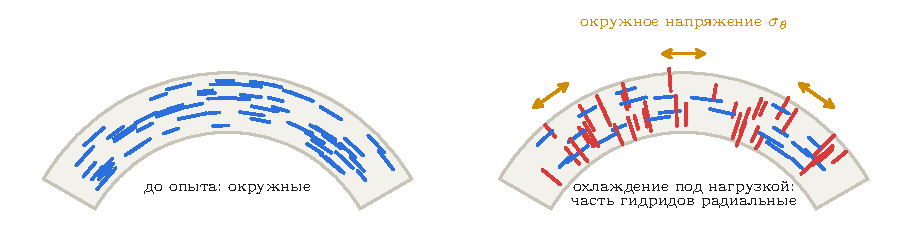
\includegraphics[width=0.85\linewidth]{f0_tube}\par
\vspace{1.5cm}
{\color{sub}Собственное изложение с рисунками, рассчитанными по формулам.\\
Опирается на классические учебники (список в приложении В), но не пересказывает их.\par}
\vfill
{\color{sub}октябрь 2026\par}
\end{titlepage}

\tableofcontents

\mainmatter
\chapter*{Введение: зачем этот фундамент}
\addcontentsline{toc}{chapter}{Введение: зачем этот фундамент}
\markboth{Введение}{Введение}

Водород, попавший в оболочку твэла из циркониевого сплава, при охлаждении выпадает в виде тонких пластинок
гидрида. Обычно они лежат вдоль окружности трубы и почти не мешают ей держать давление. Но если труба остывает под
растягивающим окружным напряжением, часть пластинок встаёт поперёк --- по радиусу (рис.~\ref{fig:f0_tube}).
Радиальные гидриды режут стенку поперёк и делают металл хрупким. Модель, ради которой написан этот текст,
предсказывает, сколько гидридов переориентируется при заданных водороде, температуре, напряжении и структуре
металла.

\fig{f0_tube}{Переориентация гидридов в сечении трубы (схема). Слева --- до опыта: пластинки гидрида (синие)
лежат вдоль окружности. Справа --- после охлаждения под окружным напряжением $\sigma_\theta$: часть пластинок
встала по радиусу (красные).}

Чтобы такую модель построить или хотя бы понять, нужно одновременно держать в голове несколько областей:
термодинамику растворов, диффузию, кристаллографию, теорию упругости, теорию зарождения и пластичность.
Каждая из них --- отдельный учебник. Здесь собрано только то, что реально работает в задаче о гидридах,
и объяснено так, чтобы было видно, \emph{почему} формулы такие, а не только \emph{какие} они.

\section*{Как устроен текст}

\begin{center}
\small
\begin{tabularx}{\linewidth}{>{\raggedright\arraybackslash}p{4.6cm}X>{\centering\arraybackslash}p{1.4cm}}
\toprule
что есть в модели & что нужно понимать & глава \\
\midrule
пределы растворимости водорода, гистерезис растворения и выпадения & энергия Гиббса, химический потенциал, растворы, общая касательная & 1, 2 \\
перенос водорода между гидридами, к растянутым местам & законы Фика, химический потенциал как движущая сила, эффект Горского & 3 \\
форма и плоскость залегания пластинок, межфазные границы & решётка ГПУ, гидриды циркония, когерентность, дислокации & 4 \\
энергия пластинки, поле напряжений вокруг неё, работа нагрузки & собственная деформация, задача Эшелби, метод Фурье & 5 \\
когда и где появляется пластинка, как растёт & классическая теория зарождения, неоднородное зарождение, рост, кинетика & 6 \\
пластическая аккомодация, память, текстура трубы & текучесть, дислокационная пластичность, текстура и факторы Кернса & 7 \\
\bottomrule
\end{tabularx}
\end{center}

Главы можно читать по порядку: каждая опирается на предыдущие. В каждой есть блоки трёх видов.
\begin{itemize}
\item \textbf{\color{circ}Интуиция} --- что происходит «на пальцах», до формул.
\item \textbf{\color{load}Главная формула} --- то, что стоит запомнить или уметь вывести.
\item \textbf{\color{hydr}Для гидридов} --- как общий результат применяется к водороду в цирконии, с числами.
\end{itemize}
В конце глав --- упражнения; ответы и подсказки собраны в приложении Б. Справочные величины для системы Zr--H
с источниками --- в приложении А. Все рисунки посчитаны по формулам этого текста (скрипты лежат в
\texttt{figs\_src/}); числа на них можно проверить самостоятельно.

\section*{Единицы и масштабы}

В задаче о гидридах встречаются энергии «на атом», «на моль» и «на кубический метр»; их полезно уметь переводить
друг в друга с ходу.
\begin{itemize}
\item Тепловая энергия: $k_BT$ на атом или $RT$ на моль. При 300\degC{} ($T = 573$~К)
  $RT \approx 4.8$~кДж/моль, $k_BT \approx 0.049$~эВ. Это мера «тепловых толчков»: барьер в $20RT$ при этой
  температуре преодолевается редко, в $2RT$ --- постоянно.
\item Концентрацию водорода в цирконии обычно дают в \emph{ppm по массе} (wppm, млн$^{-1}$): микрограммы водорода
  на грамм металла. Атомная доля $x_{\mathrm H} \approx C_{\mathrm{ppm}} \cdot 91.22 / (1.008\cdot 10^6)$, то есть
  100~ppm $\approx 0.9$~ат.\,\%.
\item Энергия на единицу объёма: 1~МДж/м$^3$ = 1~МПа. Напряжение --- это и есть плотность энергии. Поэтому
  работа нагрузки 100~МПа на деформации 7\,\% равна 7~МДж/м$^3$, и её можно прямо сравнивать с упругой энергией
  гидрида в тех же единицах (глава~5).
\item Объём гидрида на моль водорода около $10^{-5}$~м$^3$. Поэтому 1~МДж/м$^3$ гидрида $\approx 10$~Дж на моль водорода.
\end{itemize}

\chapter{Энергия Гиббса и равновесие}

\section{Что стремится к минимуму}

Изолированная система движется к максимуму энтропии: это второе начало термодинамики. Но кусок металла в печи
не изолирован --- он обменивается теплом с окружением при постоянной температуре $T$ и постоянном давлении $p$.
Если посчитать энтропию \emph{системы вместе с печью}, окажется, что её рост равносилен убыванию одной величины,
относящейся только к образцу, --- \textbf{энергии Гиббса}
\begin{equation}
G = H - TS,\qquad H = U + pV .
\end{equation}
Здесь $H$ --- энтальпия (для твёрдых тел почти то же, что внутренняя энергия: член $pV$ при атмосферном давлении
мал), $S$ --- энтропия.

\begin{idea}
Почему именно $H - TS$? Когда образец выделяет теплоту $Q$, энтропия печи растёт на $Q/T$. Выделение теплоты
означает уменьшение $H$ образца. Значит, суммарная энтропия растёт, если $\Delta S_{\text{обр}} - \Delta H/T > 0$,
то есть если $\Delta(H - TS) < 0$. Энергия Гиббса --- это энтропия Вселенной, пересчитанная на образец и взятая
со знаком минус.
\end{idea}

Два слагаемых тянут в разные стороны. Энтальпия любит порядок: атомы ставятся так, чтобы связи были
прочнее. Энтропия любит беспорядок: много способов расставить атомы. Множитель $T$ решает, кто сильнее. При
низкой температуре выигрывает энтальпия --- плотные упорядоченные фазы, соединения, выпадение второй фазы. При
высокой --- энтропия: растворы, расплавы, высокотемпературные модификации.

\section{Устойчивость, метастабильность и барьер}

Фаза устойчива при данных $T$ и $p$, если у неё наименьшая $G$ из всех доступных состояний. Однако
\emph{наименьшая} $G$ --- не единственное, что важно. На рис.~\ref{fig:f1_gibbs}б показан профиль энергии по
некоторой «координате» перестройки атомов. Состояние в локальной яме \textbf{метастабильно}: малые отклонения
возвращают его назад, и, чтобы попасть в более глубокую яму, система должна преодолеть \textbf{барьер}
$\Delta G_a$. Состояние на вершине \textbf{неустойчиво} --- любое отклонение уводит его вниз.

\fig{f1_gibbs}{а) Энергии Гиббса двух фаз в зависимости от температуры. Кривые пересекаются при $T_e$; ниже
устойчива $\alpha$, выше --- $\beta$. На расстоянии $\Delta T$ от $T_e$ разность $\Delta G$ --- движущая сила
превращения. б) Устойчивое, метастабильное и неустойчивое состояния; барьер $\Delta G_a$ держит метастабильное
состояние.}

Почти всё интересное в материаловедении --- метастабильно. Пересыщенный твёрдый раствор водорода в цирконии
после быстрого охлаждения --- метастабилен: гидрид выгоднее, но чтобы он появился, нужно преодолеть барьер
зарождения (глава~6). Скорость, с которой система переходит барьер, пропорциональна $\exp(-\Delta G_a/k_BT)$.
Отсюда два вывода, которые будут повторяться во всём тексте:
\begin{enumerate}
\item термодинамика говорит, \emph{куда} может идти процесс (знак $\Delta G$);
\item кинетика --- \emph{как быстро} (высота барьера и подвижность атомов).
\end{enumerate}

\section{Движущая сила вблизи температуры превращения}

Пусть две фазы равновесны при $T_e$: $G_\alpha(T_e) = G_\beta(T_e)$. Немного ниже, при $T = T_e - \Delta T$,
разность энергий
\[
\Delta G = \Delta H - T\,\Delta S .
\]
При $T_e$ она равна нулю, значит $\Delta S = \Delta H/T_e$. Если $\Delta H$ и $\Delta S$ слабо зависят от
температуры (так и есть в узком интервале), то
\begin{keyf}
\[
\Delta G \approx \Delta H - T\,\frac{\Delta H}{T_e} = \frac{\Delta H\,\Delta T}{T_e}.
\]
\end{keyf}
Движущая сила растёт пропорционально переохлаждению. На самой температуре равновесия её нет вовсе --- и поэтому
никакое превращение не идёт \emph{точно} при $T_e$: нужно переохлаждение (или перегрев), чтобы появилась сила,
способная оплатить барьер. Это первая встреча с идеей, которая объяснит гистерезис растворения и выпадения
гидридов (глава~2).

\section{Химический потенциал}

В сплаве атомы разных сортов могут переходить из фазы в фазу. Нужна величина, которая говорит, выгодно ли
атому сорта $i$ перейти. Это \textbf{химический потенциал}
\begin{equation}
\mu_i = \left(\frac{\partial G}{\partial n_i}\right)_{T,p,n_{j\ne i}},
\end{equation}
изменение энергии Гиббса при добавлении одного моля компонента $i$ (при неизменном прочем).

\begin{idea}
Химический потенциал --- это «давление» для атомов данного сорта. Атомы сами собой перетекают туда, где
их $\mu$ меньше, как газ --- туда, где давление ниже. Равновесие наступает, когда $\mu_i$ одинаков во всех фазах
и во всех точках. Из этого простого условия следуют и общая касательная (глава~2), и диффузия к растянутым местам
(глава~3), и сдвиг растворимости под нагрузкой (глава~6).
\end{idea}

Условие равновесия двух фаз $\alpha$ и $\beta$ по всем компонентам:
\begin{equation}
\mu_i^\alpha = \mu_i^\beta\qquad\text{для каждого } i .
\end{equation}
В двухкомпонентной системе это два уравнения. Графически --- общая касательная к кривым $G(X)$ двух фаз; к ней мы
придём в следующей главе.

\section{Масштабы энергий}

Полезно заранее держать в голове порядки величин (на моль):
\begin{center}\small
\begin{tabular}{lr}
\toprule
энергия связи атомов металла (теплота сублимации Zr) & $\sim 600$~кДж/моль \\
теплота растворения водорода в $\alpha$-Zr (из наклона TSSD, глава~2) & $\sim 40$~кДж/моль \\
тепловая энергия $RT$ при 300\degC & 4.8~кДж/моль \\
движущая сила выпадения гидрида на линии выпадения & $\sim 5$~кДж/моль H \\
упругая энергия тонкой пластинки гидрида (глава~5) & $\sim 3$~кДж/моль H \\
работа нагрузки 100~МПа на несоответствии гидрида & $\sim 0.07$~кДж/моль H \\
\bottomrule
\end{tabular}
\end{center}
Последние три строки --- суть всей задачи о переориентации: работа нагрузки в десятки раз меньше движущей силы и
упругой энергии, и всё же она решает, как ляжет пластинка. Почему так получается --- главы~5 и 6.

\begin{exercise}
Две фазы равновесны при $T_e = 1000$~К, теплота превращения $\Delta H = 10$~кДж/моль. Оцените движущую силу при
переохлаждении на 10 и на 100~К. Во сколько раз она меньше $RT$ в каждом случае?
\end{exercise}

\begin{exercise}
Скорость перехода через барьер пропорциональна $e^{-\Delta G_a/RT}$. Барьер 120~кДж/моль. Во сколько раз быстрее
процесс при 400\degC, чем при 300\degC?
\end{exercise}

\begin{exercise}
Покажите, что из условия $\dd G = V\dd p - S\dd T$ для двух равновесных фаз следует уравнение Клапейрона
$\dd p/\dd T = \Delta H/(T\Delta V)$. Как, по аналогии, напряжение $\sigma$, совершающее работу на деформации
превращения $\eps^*$, сдвигает температуру равновесия? (К этому вопросу мы вернёмся в главе~6.)
\end{exercise}

\chapter{Растворы, диаграммы состояния и водород в цирконии}

\section{Идеальный раствор: энтропия перемешивания}

Возьмём $N$ узлов решётки и рассадим на них $N_B = XN$ атомов сорта $B$ и $N_A = (1-X)N$ атомов $A$. Число
различимых расстановок $W = N!/(N_A!\,N_B!)$. По Больцману энтропия $S = k_B\ln W$; с формулой Стирлинга
$\ln N! \approx N\ln N - N$ получаем на моль
\begin{equation}
\Delta S_{\text{mix}} = -R\,\bigl[X\ln X + (1-X)\ln(1-X)\bigr] .
\end{equation}
Если атомы $A$ и $B$ «безразличны» друг к другу (энергия связи $A$--$B$ равна средней из $A$--$A$ и $B$--$B$),
теплота смешения равна нулю, и
\begin{equation}
\Delta G_{\text{mix}} = RT\,\bigl[X\ln X + (1-X)\ln(1-X)\bigr] < 0 .
\end{equation}
Это \textbf{идеальный раствор}. Смешение выгодно всегда, при любом составе: энтропия выигрывает «бесплатно».

\begin{idea}
У функции $X\ln X$ производная при $X\to 0$ уходит в $-\infty$. Значит, \emph{первые} атомы примеси растворяются
с огромным выигрышем энтропии. Поэтому абсолютно чистых веществ не бывает и растворимость любой примеси, пусть
крошечная, всегда больше нуля.
\end{idea}

\section{Регулярный раствор: когда соседи не безразличны}

Пусть энергии связей различаются. В простейшей модели каждый атом взаимодействует только с $z$ ближайшими
соседями, а расстановка остаётся случайной. Тогда теплота смешения
\begin{equation}
\Delta H_{\text{mix}} = \Omega X(1-X),\qquad
\Omega = N_A z\Bigl[\eps_{AB} - \tfrac12(\eps_{AA}+\eps_{BB})\Bigr],
\end{equation}
и $\Delta G_{\text{mix}} = \Omega X(1-X) + RT[X\ln X + (1-X)\ln(1-X)]$. Знак $\Omega$ решает всё
(рис.~\ref{fig:f2_mixing}):
\begin{itemize}
\item $\Omega < 0$: разноимённые соседи выгодны, раствор ещё устойчивее идеального, при низких $T$ возможно упорядочение;
\item $\Omega > 0$: выгоднее одноимённые соседи. Пока $T$ высока, энтропия держит раствор однородным; при
  $\Omega/RT > 2$ на кривой $G(X)$ появляются две ямы --- раствор хочет разделиться на две фазы.
\end{itemize}

\fig{f2_mixing}{а) Энергия смешения регулярного раствора в единицах $RT$ при разных $\Omega/RT$. При
$\Omega/RT > 2$ появляется двойная яма. б) Для $\Omega/RT = 2.5$: энтальпия (красная) против смешения,
энтропийный член (синий) --- за; сумма (чёрная) имеет два минимума.}

Химический потенциал компонента $B$ в регулярном растворе
\begin{equation}
\mu_B = G_B^0 + \Omega(1-X)^2 + RT\ln X .
\end{equation}
Для разбавленного раствора ($X\to 0$) член $\Omega(1-X)^2\to\Omega$ --- константа, и
\begin{keyf}[Разбавленный раствор]
\[
\mu_B \approx \mu_B^{\infty} + RT\ln X .
\]
\end{keyf}
Это закон Генри: в разбавленном растворе химический потенциал растёт как логарифм концентрации, что бы ни
происходило с атомами в деталях. Водород в $\alpha$-цирконии --- как раз такой случай: даже 600~ppm --- это
5~ат.\,\%. Вся термодинамика растворимости гидридов держится на одной этой формуле.

\section{Расслоение: бинодаль, спинодаль, общая касательная}

Если кривая $G(X)$ имеет две ямы, раствор состава $X_0$ между ними может понизить энергию, распавшись на две
части с составами $X_1$ и $X_2$. Энергия смеси лежит на \emph{хорде}, соединяющей точки кривой, и наилучшая
хорда --- \textbf{общая касательная} (рис.~\ref{fig:f2_gap}б). В точках касания одинаков наклон
$\partial G/\partial X$; это и есть условие равенства химических потенциалов обоих компонентов в двух фазах.

\begin{keyf}[Общая касательная и правило рычага]
Равновесные составы фаз $X_1$, $X_2$ --- точки касания общей касательной. Доли фаз в сплаве состава $X_0$:
\[
f_2 = \frac{X_0 - X_1}{X_2 - X_1},\qquad f_1 = 1 - f_2 .
\]
\end{keyf}

Если провести такое построение при каждой температуре, точки касания образуют \textbf{бинодаль} --- границу
двухфазной области на диаграмме состояния (рис.~\ref{fig:f2_gap}а). Внутри неё есть ещё одна линия ---
\textbf{спинодаль}, где кривизна $\partial^2G/\partial X^2$ меняет знак:
\begin{equation}
\frac{\partial^2 G}{\partial X^2} = -2\Omega + \frac{RT}{X(1-X)} = 0
\quad\Rightarrow\quad X(1-X) = \frac{RT}{2\Omega},\qquad T_c = \frac{\Omega}{2R}.
\end{equation}

\fig{f2_gap}{а) Купол расслоения регулярного раствора: бинодаль (чёрная) и спинодаль (красная пунктирная).
Между ними раствор метастабилен --- для распада нужно зарождение; внутри спинодали распад идёт без барьера.
б) Сечение при $T = 0.7\,T_c$: общая касательная (золотая) и точки перегиба (красные квадраты).}

\begin{idea}
Почему между бинодалью и спинодалью нужен барьер? Там кривая $G(X)$ выпукла вниз: \emph{малое} расслоение
(состав чуть больше и чуть меньше среднего) энергию повышает. Выигрыш появляется, только если сразу возникает
кусочек совсем другого состава --- зародыш новой фазы. Внутри спинодали кривая выпукла вверх, и любое малое
колебание состава растёт само. Выпадение гидридов --- случай первого типа: гидрид по составу и решётке
совсем не похож на раствор, поэтому без зарождения он не появится.
\end{idea}

\section{Растворимость второй фазы}

Теперь самое важное для нас. Пусть вторая фаза --- почти стехиометрическое соединение, например гидрид
$\mathrm{ZrH}_x$ с $x \approx 1.6$. Его кривая $G(X)$ --- узкая глубокая яма около $X_\delta \approx 0.62$
(рис.~\ref{fig:f2_tangent}). Общая касательная к ней и к кривой твёрдого раствора касается раствора в точке
$X_e$ --- это и есть \textbf{предел растворимости}.

\begin{figure}[htbp]\centering
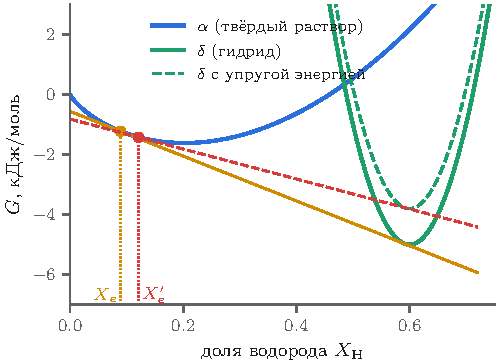
\includegraphics[width=0.62\linewidth]{f2_tangent}
\caption{Растворимость соединения в твёрдом растворе (схема). Общая касательная (золотая) к раствору $\alpha$ и
гидриду $\delta$ касается раствора в точке $X_e$. Если энергия гидрида выше (пунктир: упругая энергия
несоответствия, малый размер), касательная круче и растворимость $X_e'$ больше.}
\label{fig:f2_tangent}
\end{figure}

Посчитаем $X_e$. В равновесии химический потенциал водорода одинаков в растворе и в гидриде. В разбавленном
растворе $\mu_{\mathrm H}^\alpha = \mu_{\mathrm H}^{\infty} + RT\ln X$; в гидриде он почти не зависит от состава.
Пусть $\Delta G^0 = \Delta H^0 - T\Delta S^0$ --- изменение энергии при переводе моля водорода из гидрида в
раствор (при стандартной концентрации). Тогда $RT\ln X_e = -\Delta G^0$, и
\begin{keyf}[Предел растворимости]
\[
X_e = \exp\!\Bigl(\frac{\Delta S^0}{R}\Bigr)\exp\!\Bigl(-\frac{\Delta H^0}{RT}\Bigr) \equiv A\,e^{-Q/RT}.
\]
\end{keyf}
В координатах $\ln C$ против $1/T$ это прямая; её наклон даёт теплоту растворения $Q$, отрезок --- энтропийный
множитель $A$. Именно так и записывают экспериментальные линии растворимости водорода в цирконии.

\section{Водород в цирконии: две линии вместо одной}

Опыт (дифференциальная сканирующая калориметрия, дилатометрия, дифракция) даёт не одну линию растворимости, а
две (рис.~\ref{fig:f2_tss}):
\begin{itemize}
\item \textbf{TSSD} (terminal solid solubility for dissolution) --- при нагреве гидриды полностью растворяются,
  когда концентрация в растворе достигает этой линии;
\item \textbf{TSSP} (for precipitation) --- при охлаждении гидриды начинают выпадать заметно ниже, при концентрации
  на этой линии.
\end{itemize}

\fig{f2_tss}{а) Пределы растворимости водорода в сплаве Э635: растворение (TSSD) и выпадение (TSSP), линии
вида $\lg C = b - k\cdot 1000/T$ по данным ДСК (Плясов и др., 2023). Пунктир --- путь образца со 160~ppm:
при нагреве гидриды растворяются полностью при 394\degC, при охлаждении начинают выпадать только при 311\degC.
б) Те же линии в аррениусовых координатах: прямые с теплотами около 43 и 32~кДж/моль.}

Между линиями --- полоса гистерезиса шириной около 80\degC. Откуда она? Вернёмся к рис.~\ref{fig:f2_tangent}.
Новому гидриду, чтобы появиться, приходится «заплатить» сверх табличной энергии соединения:
\begin{itemize}
\item \textbf{упругую энергию несоответствия}: гидрид объёмнее циркония на 17\,\%, и матрица вокруг него
  деформирована (глава~5);
\item \textbf{работу пластической аккомодации}: часть несоответствия снимается пластическим течением, которое тоже
  требует работы (глава~7);
\item \textbf{энергию межфазной границы} и вообще барьер зарождения (глава~6).
\end{itemize}
Каждая такая добавка $\Delta g$ (на моль водорода) поднимает кривую гидрида, и растворимость, с которой он
равновесен, растёт в $e^{\Delta g/RT}$ раз:
\begin{equation}
\frac{C_\TSSP}{C_\TSSD} = \exp\Bigl(\frac{\Delta g}{RT}\Bigr)
\quad\Rightarrow\quad
\Delta g = RT\ln\frac{C_\TSSP}{C_\TSSD} .
\end{equation}
При растворении всё наоборот: старый гидрид уже окружён релаксированной (пластически деформированной) матрицей,
лишней энергии у него почти нет, и он растворяется близко к «истинному» равновесию.

\begin{zrbox}
Для Э635 при 300\degC: $C_\TSSD \approx 45$~ppm, $C_\TSSP \approx 141$~ppm, отношение 3.1. Значит, на линии
выпадения раствор пересыщен на $\Delta g = RT\ln 3.1 \approx 5.5$~кДж на моль водорода. В главе~5 мы увидим, что
одна только упругая энергия тонкой пластинки гидрида около 3~кДж/моль~H --- того же порядка. Остальное
--- пластичность и барьер зарождения. Линия TSSP к тому же частично \emph{кинетическая}: она смещается со скоростью
охлаждения и с тем, до какой температуры образец нагревали (сохранились ли следы старых гидридов).
\end{zrbox}

\section{Диаграмма Zr--H со стороны циркония}

Полная диаграмма Zr--H сложна: несколько гидридов ($\gamma$-ZrH, $\delta$-ZrH$_{\sim1.6}$, $\varepsilon$-ZrH$_2$),
высокотемпературная $\beta$-фаза, эвтектоид. Для оболочек важен только угол со стороны циркония
(рис.~\ref{fig:f2_zrh}):
\begin{itemize}
\item $\alpha$ --- твёрдый раствор водорода в ГПУ цирконии;
\item $\alpha+\delta$ --- раствор плюс гидрид; граница --- линия растворимости (TSSD);
\item $\beta$ --- ОЦК цирконий; водород её стабилизирует, поэтому область $\alpha+\beta$ клином уходит вниз;
\item эвтектоид при $\approx 550$\degC: $\beta \to \alpha + \delta$. Растворимость в $\alpha$ там максимальна,
  $\approx 6$~ат.\,\% (около 690~ppm).
\end{itemize}

\begin{figure}[htbp]\centering
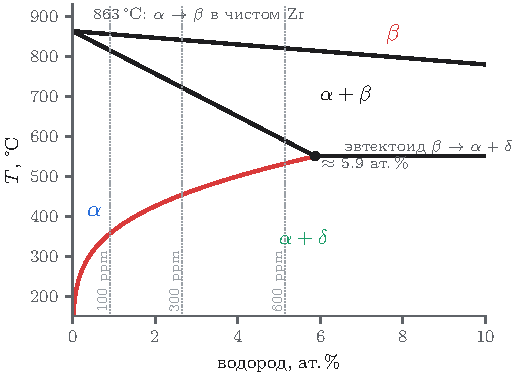
\includegraphics[width=0.6\linewidth]{f2_zrh}
\caption{Угол диаграммы Zr--H со стороны циркония (схема; сольвус $\alpha/(\alpha+\delta)$ --- по линии TSSD,
остальные границы условно прямыми). Вертикальные пунктиры --- 100, 300 и 600~ppm водорода.}
\label{fig:f2_zrh}
\end{figure}

\begin{warnbox}
Сплавы (Nb, Sn, Fe, O) немного сдвигают линии, а линия выпадения зависит от режима охлаждения. Поэтому для
конкретного материала линии берут из его собственных измерений, а не из общей диаграммы.
\end{warnbox}

\section{Сколько выпадает гидрида}

По правилу рычага при комнатной температуре почти весь водород сидит в гидриде (растворимость там --- доли ppm).
В $\delta$-ZrH$_{1.66}$ водорода $\approx 1.8$\,\% по массе (18\,000~ppm). Значит, при 160~ppm массовая доля
гидрида $160/18\,000 \approx 0.9\,\%$, а объёмная --- около 1\,\% (гидрид менее плотен). На шлифе после травления
гидриды кажутся занимающими 7--12\,\% площади --- травление сильно расширяет их следы. Об этом стоит помнить,
сравнивая снимки с расчётом.

\begin{exercise}
Выведите выражение для $\mu_B$ регулярного раствора, продифференцировав $G = (1-X)G_A + XG_B + \Delta G_{\text{mix}}$.
Проверьте, что при $X\to 0$ получается закон Генри.
\end{exercise}

\begin{exercise}
Для линии $\lg C = 5.56 - 2240/T$ найдите теплоту растворения $Q$ в кДж/моль и температуру полного растворения
для 100, 300 и 600~ppm.
\end{exercise}

\begin{exercise}
Пользуясь линиями Э635, постройте $\Delta g(T) = RT\ln(C_\TSSP/C_\TSSD)$ от 200 до 400\degC. Растёт она или падает с
температурой? Как это согласуется с тем, что пластичность легче при высокой температуре?
\end{exercise}

\begin{exercise}
Образец с 300~ppm нагрели до 400\degC. Сколько водорода осталось в нерастворённых гидридах? При какой температуре
начнётся выпадение при охлаждении?
\end{exercise}

\chapter{Диффузия}

\section{Прыжки атомов и случайное блуждание}

Атом в кристалле большую часть времени колеблется около своего места и лишь изредка, когда тепловая флуктуация
даёт ему энергию $\Delta G_m$, перепрыгивает в соседнюю позицию. Частота прыжков
\begin{equation}
\Gamma = \nu\, e^{-\Delta G_m/k_BT},
\end{equation}
где $\nu\sim10^{13}$~с$^{-1}$ --- частота колебаний. Водород в цирконии --- атом внедрения: он сидит в
тетраэдрических междоузлиях и прыгает между ними, не нуждаясь в вакансиях. Поэтому он очень подвижен.

Каждый прыжок --- в случайную сторону. После $n$ прыжков длиной $a$ средний сдвиг равен нулю, а средний
\emph{квадрат} сдвига растёт линейно (рис.~\ref{fig:f3_walk}):
\begin{equation}
\langle x^2\rangle = n a^2 \quad(\text{одномерно}),\qquad n = \Gamma t .
\end{equation}
Определим коэффициент диффузии так, чтобы $\langle x^2\rangle = 2Dt$ в одном измерении ($6Dt$ в трёх). Тогда
\begin{keyf}[Коэффициент диффузии]
\[
D = \frac{\Gamma_{\text{пол}} a^2}{6} = D_0\,e^{-Q/RT},
\]
где $\Gamma_{\text{пол}}$ --- полная частота прыжков во всех направлениях, $Q$ --- энергия активации миграции.
\end{keyf}

\fig{f3_walk}{а) Траектории пяти атомов по 400 случайных прыжков: каждая непредсказуема, но типичный уход ---
порядка $\sqrt n\,a$ (пунктирная окружность). б) Распределение смещений 20\,000 одномерных блужданий после $n$
прыжков: гистограммы ложатся на гауссианы с $\langle x^2\rangle = na^2$.}

\begin{idea}
Главное следствие: расстояние растёт как \emph{корень} из времени. Чтобы уйти вдвое дальше, нужно вчетверо
больше времени. Диффузионная длина $\sqrt{Dt}$ --- универсальная мерка «куда успеет дойти атом за время $t$».
\end{idea}

\section{Законы Фика}

На макроуровне случайные прыжки дают поток из мест, где атомов больше, туда, где их меньше (первый закон Фика):
\begin{equation}
\mathbf J = -D\,\nabla c .
\end{equation}
Сохранение числа атомов $\partial c/\partial t = -\nabla\cdot\mathbf J$ даёт второй закон:
\begin{keyf}[Уравнение диффузии]
\[
\frac{\partial c}{\partial t} = \nabla\cdot(D\nabla c) \;=\; D\,\nabla^2 c\quad(D = \text{const}).
\]
\end{keyf}

Два решения, которые стоит знать наизусть (рис.~\ref{fig:f3_profiles}):
\begin{itemize}
\item \textbf{тонкий слой} количества $M$ в точке $x=0$ расплывается гауссианой
  \[c(x,t) = \frac{M}{\sqrt{4\pi Dt}}\,e^{-x^2/4Dt};\]
\item \textbf{постоянная концентрация $c_s$ на поверхности} полубесконечного тела:
  \[c(x,t) = c_s\,\operatorname{erfc}\Bigl(\frac{x}{2\sqrt{Dt}}\Bigr).\]
  На глубине $x = 2\sqrt{Dt}$ концентрация уже
  $0.16\,c_s$.
\end{itemize}

\fig{f3_profiles}{а) Тонкий слой расплывается гауссианой. б) Профиль от поверхности с постоянной концентрацией
--- функция erfc; точки --- глубина $2\sqrt{Dt}$, где концентрация 16\,\% от поверхностной. Во всех решениях
масштаб длины --- $\sqrt{Dt}$.}

\section{Водород в цирконии: насколько он подвижен}

Для водорода в $\alpha$-цирконии (Kearns, 1972)
\[
D \approx 7.9\cdot10^{-7}\exp\Bigl(-\frac{44.4~\text{кДж/моль}}{RT}\Bigr)~\text{м}^2/\text{с}.
\]
При 300\degC{} $D\approx 7\cdot10^{-11}$~м$^2$/с, при 400\degC{} --- $3\cdot10^{-10}$. За минуту водород
проходит около 0.1~мм, за час --- 0.5--1~мм, то есть всю стенку трубы (рис.~\ref{fig:f3_dh}).

\begin{figure}[htbp]\centering
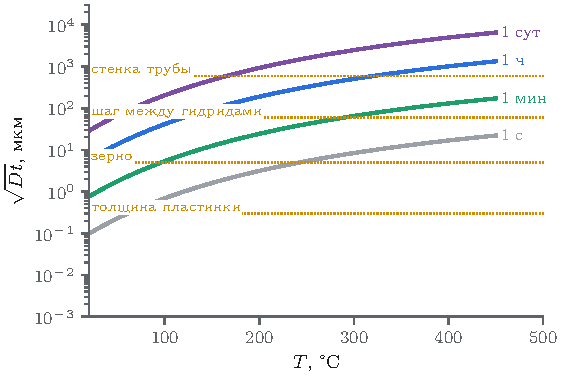
\includegraphics[width=0.66\linewidth]{f3_dh}
\caption{Диффузионная длина водорода в $\alpha$-Zr $\sqrt{Dt}$ от температуры для 1~с, 1~мин, 1~ч и 1~сут против
характерных размеров структуры. При охлаждении 0.5--1\degC/мин водород за время прохода каждого градуса успевает
уйти на десятки микрометров --- больше расстояния между гидридами.}
\label{fig:f3_dh}
\end{figure}

\begin{zrbox}
Отсюда важный вывод для модели. При обычных скоростях охлаждения водород успевает выравнивать концентрацию на
масштабе зёрен и между соседними гидридами. Выпадение ограничено не подводом водорода издалека, а тем, где и
когда удаётся \emph{зародиться} пластинке. Зато на масштабе ниже сотни микрометров диффузия решает, какой из
соседних зародышей «перехватит» водород и вырастет.
\end{zrbox}

\section{Движущая сила --- градиент химического потенциала}

Закон Фика в форме $\mathbf J = -D\nabla c$ --- частный случай. Атомы на самом деле текут вниз по
\emph{химическому потенциалу}:
\begin{equation}
\mathbf J = -\frac{D\,c}{RT}\,\nabla\mu .
\end{equation}
Для разбавленного раствора $\mu = \mu^\infty + RT\ln c$, и $\nabla\mu = RT\nabla c/c$ --- возвращаемся к Фику. Но
если на $\mu$ влияет что-то ещё, поток может идти даже \emph{против} градиента концентрации («восходящая
диффузия»).

Самый важный для нас пример --- \textbf{напряжения}. Атом водорода расширяет решётку на свой парциальный мольный
объём $\bar V_{\mathrm H}\approx 1.7$~см$^3$/моль. В растянутой области (гидростатическое напряжение
$\sigma_h = (\sigma_{11}+\sigma_{22}+\sigma_{33})/3 > 0$) поместить его легче: работа $-\bar V_{\mathrm H}\sigma_h$
понижает его потенциал:
\begin{equation}
\mu = \mu^\infty + RT\ln c - \bar V_{\mathrm H}\,\sigma_h .
\end{equation}

\begin{keyf}[Диффузия в поле напряжений]
\[
\mathbf J = -D\Bigl(\nabla c - \frac{c\,\bar V_{\mathrm H}}{RT}\nabla\sigma_h\Bigr),
\qquad\text{в равновесии}\quad c = c_0\exp\Bigl(\frac{\bar V_{\mathrm H}\sigma_h}{RT}\Bigr).
\]
\end{keyf}

Перетекание водорода в растянутые места называют \textbf{эффектом Горского}. Он тем сильнее, чем ниже
температура и больше напряжение (рис.~\ref{fig:f3_stress}). При 300\degC{} и $\sigma_h = 300$~МПа концентрация
выше на 11\,\%. У вершины трещины, где $\sigma_h$ доходит до 2--3 пределов текучести, --- в полтора раза.
На этом стоит механизм замедленного гидридного растрескивания: водород стекается к вершине трещины, там
выпадает гидрид, гидрид трескается, трещина продвигается.

\fig{f3_stress}{а) Равновесное обогащение водородом перед вершиной трещины ($K = 10$~МПа$\sqrt{\text{м}}$,
плоская деформация). Вблизи вершины напряжение ограничено пластичностью ($\sigma_h\approx3\sigma_y$), поэтому
обогащение выходит на полку. б) Обогащение $c/c_0$ от гидростатического напряжения при трёх температурах.}

\begin{zrbox}
Внешнее окружное напряжение 100~МПа в трубе само по себе меняет концентрацию всего на 1--2\,\%: водород
перераспределяется слабо. Важнее \emph{локальные} напряжения у торцов уже выпавших гидридов --- там $\sigma_h$
доходит до сотен МПа (глава~5), и водород стекается к торцам. Так поле напряжений и диффузия вместе
выстраивают гидриды в цепочки.
\end{zrbox}

Есть и \textbf{термодиффузия} (эффект Соре): в градиенте температуры водород уходит в холодную сторону. В твэле
внешняя поверхность оболочки холоднее, и водород копится у неё --- так образуется гидридный обод. Формально это
ещё один вклад в $\mu$, пропорциональный теплоте переноса $Q^*$.

\section{Как решать уравнение диффузии на компьютере}

Простейшая \textbf{явная схема} на сетке с шагом $\Delta x$:
\begin{equation}
c_i^{n+1} = c_i^n + r\,\bigl(c_{i+1}^n - 2c_i^n + c_{i-1}^n\bigr),\qquad r = \frac{D\,\Delta t}{\Delta x^2}.
\end{equation}
Она устойчива, только если $r \le 1/2$ в одномерном случае ($1/4$ на квадратной сетке в 2D). При большем шаге
самая короткая гармоника (пила с периодом $2\Delta x$) умножается за шаг на $|1-4r| > 1$ и растёт без предела
(рис.~\ref{fig:f3_numerics}).

\fig{f3_numerics}{Явная схема для уравнения диффузии после 80 шагов. а) $r = 0.45$: совпадает с точным решением.
б) $r = 0.51$: чуть выше предела, и из ошибок округления уже выросла пила, которая дальше растёт
экспоненциально.}

\begin{idea}
Почему именно $1/2$? Явная схема переносит за шаг долю $r$ вещества в каждого соседа. Если $r > 1/2$, клетка
отдаёт больше, чем имела, --- и концентрация «перескакивает» через равновесие, раскачиваясь всё сильнее.
\end{idea}

Модель гидридов решает диффузию \textbf{спектральным методом}: поле раскладывается по гармоникам Фурье
$e^{i\mathbf k\cdot\mathbf x}$, и каждая затухает точно как $e^{-Dk^2\Delta t}$. Для постоянного $D$ на
периодической сетке это точное решение при любом шаге по времени. Тот же приём --- и для упругих полей
(глава~5).

\begin{exercise}
Оцените время, за которое водород при 350\degC{} выравнивает концентрацию по толщине стенки 0.65~мм.
А по расстоянию между гидридами 50~мкм?
\end{exercise}

\begin{exercise}
Выведите равновесное распределение $c\propto e^{\bar V\sigma_h/RT}$, приравняв поток нулю. Оцените обогащение при
$\sigma_h = 600$~МПа (у торца гидрида) при 300\degC.
\end{exercise}

\begin{exercise}
Подставьте в явную схему пробное решение $c_i^n = g^n e^{ik i\Delta x}$ и найдите множитель $g(k)$. Докажите, что
$|g|\le1$ для всех $k$ при $r\le1/2$.
\end{exercise}

\chapter{Кристаллы, дефекты и границы}

\section{Гексагональная решётка циркония}

Ниже 863\degC{} цирконий имеет \textbf{гексагональную плотноупакованную} (ГПУ) решётку --- $\alpha$-Zr.
Её ячейка --- шестигранная призма (рис.~\ref{fig:f4_hcp}а) с параметрами $a \approx 0.323$~нм в основании и
$c\approx 0.515$~нм по высоте; отношение $c/a\approx1.593$ немного меньше идеального $\sqrt{8/3}=1.633$.

Плоскости и направления в ГПУ удобно обозначать четырьмя индексами Миллера--Браве $(hkil)$ с $i = -(h+k)$:
три оси $a_1, a_2, a_3$ в базисной плоскости под 120\textdegree{} и ось $c$. Лишний индекс нужен, чтобы
одинаковые по симметрии плоскости и выглядели одинаково. Важнейшие плоскости:
\begin{itemize}
\item \textbf{базисная} $(0001)$ --- перпендикулярна оси $c$;
\item \textbf{призматические} $\{10\bar10\}$ --- боковые грани призмы, параллельны $c$;
\item \textbf{пирамидальные} $\{10\bar1l\}$ --- наклонные. Плоскость $\{10\bar17\}$, около которой лежат
  гидриды, всего на 15\textdegree{} отклонена от базисной.
\end{itemize}

\fig{f4_hcp}{а) Ячейка ГПУ $\alpha$-Zr: базисная плоскость $(0001)$ (синяя), призматическая $\{10\bar10\}$
(красная), оси $a_1$--$a_3$ и $c$. б) Пластинка $\delta$-гидрида на плоскости, близкой к базисной: в плоскости
пластинки гидрид шире матрицы на $\approx4.6\,\%$, поперёк неё --- на $\approx7.2\,\%$.}

\begin{idea}
ГПУ решётка сильно \emph{анизотропна}: свойства вдоль $c$ и поперёк различаются. Тепловое расширение вдоль
$c$ заметно больше, чем в базисной плоскости. Скольжение дислокаций легко идёт по призматическим плоскостям и
трудно --- с компонентой вдоль $c$. Поэтому то, как ориентированы оси $c$ зёрен (текстура, глава~7), определяет и
прочность трубы, и то, как в ней лягут гидриды.
\end{idea}

\section{Гидриды циркония}

У циркония несколько гидридов:
\begin{itemize}
\item $\delta$-ZrH$_{1.5\ldots1.7}$ --- основной в оболочках. Решётка гранецентрированная кубическая (типа
  флюорита), $a\approx0.478$~нм. Водород занимает тетраэдрические пустоты.
\item $\gamma$-ZrH --- гранецентрированная тетрагональная; метастабильная, появляется при быстром охлаждении.
\item $\varepsilon$-ZrH$_2$ --- при очень высоком водороде.
\end{itemize}
$\delta$-гидрид выпадает с ориентационным соотношением $(0001)_\alpha\parallel\{111\}_\delta$,
$\langle11\bar20\rangle_\alpha\parallel\langle110\rangle_\delta$: плотноупакованные плоскости обеих решёток
параллельны. При таком сопряжении гидрид шире матрицы на $\eps_a\approx4.6\,\%$ в базисной плоскости и на
$\eps_c\approx7.2\,\%$ вдоль оси $c$; объём больше на $\approx17\,\%$ (Carpenter, 1973).

\begin{zrbox}
Гидрид, видимый на шлифе как одна линия длиной в десятки--сотни микрометров, на самом деле --- пачка тонких
\emph{микропластинок} толщиной 0.1--1~мкм и длиной в единицы микрометров. Они лежат около $\{10\bar17\}$ внутри зёрен
и цепляются друг за друга, переходя из зерна в зерно. Модель работает именно с микропластинками, а «макрогидрид»
--- результат их коллективного расположения.
\end{zrbox}

\section{Точечные дефекты}

Даже идеальный кристалл при $T>0$ содержит \textbf{вакансии} --- пустые узлы. Их равновесная доля
\begin{equation}
c_v = e^{S_f/k_B}\,e^{-H_f/k_BT},
\end{equation}
$H_f\sim1$--2~эВ, у точки плавления $c_v\sim10^{-4}$. Образование вакансии стоит энергии, но приносит
энтропию --- та же борьба $H$ и $TS$, что и в главе~1. Атомы \textbf{внедрения} (водород, кислород, углерод)
сидят в пустотах между узлами. Именно поэтому водород не нуждается в вакансиях, чтобы двигаться.

\section{Дислокации}

Пластическая деформация металла идёт не сдвигом целых атомных плоскостей разом (на это нужны напряжения порядка
$\mu/10$, в сотни раз больше реальных), а движением \textbf{дислокаций} --- линейных дефектов, вдоль которых
одна часть кристалла уже сдвинута относительно другой.

Проще всего представить \textbf{краевую дислокацию}: в кристалл сверху вставлена лишняя полуплоскость атомов,
обрывающаяся на плоскости скольжения (рис.~\ref{fig:f4_dislocation}а). Сдвиг, который несёт дислокация, задаёт
\textbf{вектор Бюргерса} $\mathbf b$; в цирконии для лёгкого скольжения $\mathbf b = \tfrac13\langle11\bar20\rangle$,
$|\mathbf b| = a$. Когда дислокация проходит через кристалл, верхняя половина сдвигается на $\mathbf b$.

\fig{f4_dislocation}{а) Краевая дислокация: над плоскостью скольжения вставлена лишняя полуплоскость (красные
атомы), соседние столбцы раздвинуты. б) Напряжение $\sigma_{xx}$ вокруг неё (изотропная теория упругости): над
плоскостью скольжения --- сжатие, под ней --- растяжение; убывает как $1/r$.}

Вокруг дислокации решётка искажена, и её поле напряжений спадает как $1/r$:
\begin{equation}
\sigma_{xx} = -\frac{\mu b}{2\pi(1-\nu)}\,\frac{y\,(3x^2+y^2)}{(x^2+y^2)^2}.
\end{equation}
Энергия дислокации на единицу длины $\approx \mu b^2/2$ --- несколько эВ на каждое межатомное расстояние. Поэтому
дислокации никогда не находятся в равновесии: они появляются при деформации и остаются, пока их не уберёт отжиг.

\begin{zrbox}
Дислокации важны для гидридов трижды:
\begin{itemize}
\item в растянутой области под краевой дислокацией водороду «просторнее» (глава~3), и туда он стекается ---
  дислокации служат местами зарождения гидридов;
\item гидрид при выпадении сам рождает дислокации вокруг себя: его несоответствие слишком велико, чтобы матрица
  выдержала его упруго (глава~7);
\item эти дислокации остаются после растворения гидрида и «помнят» его место --- при следующем охлаждении гидрид
  выпадает там же. Это \textbf{эффект памяти}.
\end{itemize}
\end{zrbox}

\section{Межфазные границы}

Граница между матрицей и выделением бывает трёх типов (рис.~\ref{fig:f4_interfaces}).
\begin{itemize}
\item \textbf{Когерентная}: атомные плоскости непрерывно переходят через границу; несоответствие решёток
  снимается упругим искажением. Энергия границы мала (0.05--0.2~Дж/м$^2$), но упругая энергия велика и растёт с
  объёмом выделения.
\item \textbf{Полукогерентная}: несоответствие частично снято \textbf{дислокациями несоответствия}, по одной на
  каждые $b/\delta$ плоскостей, где $\delta = (a_\beta - a_\alpha)/a_\alpha$. Энергия границы выше (0.2--0.5).
\item \textbf{Некогерентная}: решётки никак не сопряжены. Энергия границы велика (0.5--1), зато упругое поле
  почти снимается.
\end{itemize}

\fig{f4_interfaces}{Типы межфазных границ: а) когерентная --- решётка выделения подстроена под матрицу;
б) полукогерентная --- периодические дислокации несоответствия ($\perp$); в) некогерентная.}

\begin{idea}
Выделение выбирает компромисс между энергией границы (растёт как площадь, $\propto r^2$) и упругой энергией
(растёт как объём, $\propto r^3$). Маленький зародыш почти всегда когерентен: граница дешёвая, а упругая энергия
при малом объёме ещё невелика. Большой гидрид теряет когерентность, рождая дислокации.
\end{idea}

\section{Границы зёрен}

Металл трубы --- поликристалл из зёрен в несколько микрометров с разной ориентацией решётки. На стыке двух зёрен
--- \textbf{граница зерна}. При малой разориентации $\theta$ это просто стенка дислокаций, и её энергия растёт по
формуле Рида--Шокли $\gamma = \gamma_m(\theta/\theta_m)\bigl(1-\ln(\theta/\theta_m)\bigr)$. При $\theta\gtrsim15^\circ$
дислокации сливаются, и энергия выходит на плато $\gamma_m\approx0.5$--1~Дж/м$^2$ с провалами у особых
разориентаций (рис.~\ref{fig:f4_gb}).

\begin{figure}[htbp]\centering
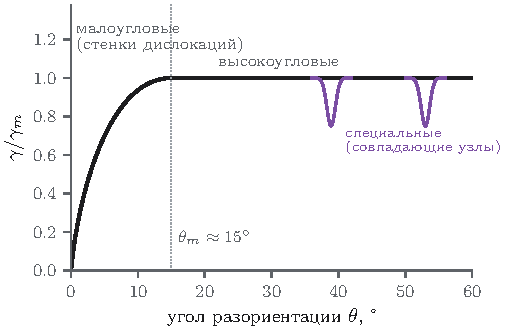
\includegraphics[width=0.6\linewidth]{f4_gb}
\caption{Энергия границы зерна от угла разориентации: рост по Риду--Шокли для малоугловых границ, плато для
высокоугловых, провалы у специальных разориентаций (совпадающих узлов) --- условно.}
\label{fig:f4_gb}
\end{figure}

\begin{zrbox}
Границы зёрен --- готовые места для зарождения: часть энергии границы «уходит в дело», когда на ней вырастает
выделение (глава~6). Гидриды часто выпадают на границах, и межзёренные гидриды могут быть ориентированы иначе, чем
внутризёренные, привязанные к базисной плоскости своего зерна (Qin и др., 2011; Wang и др., 2019). Это ещё один
путь к радиальным гидридам, когда внутри зёрен им мешает текстура.
\end{zrbox}

\begin{exercise}
Найдите угол между нормалью к плоскости $(10\bar17)$ и осью $c$ в ГПУ с $c/a = 1.593$. (Подсказка: для плоскости
$(hkil)$ угол $\varphi$ с базисом даёт $\operatorname{tg}\varphi = \tfrac{2}{\sqrt3}\,\tfrac{c}{a}\,\sqrt{h^2+hk+k^2}/l$.)
\end{exercise}

\begin{exercise}
Объёмное несоответствие гидрида 17\,\%. Сколько это в линейном несоответствии, если считать его изотропным? Через
сколько межплоскостных расстояний пришлось бы ставить дислокацию несоответствия, чтобы снять его полностью?
\end{exercise}

\begin{exercise}
Оцените энергию дислокации на единицу длины при $\mu = 33$~ГПа, $b = 0.323$~нм. Сколько это в эВ на межатомное
расстояние?
\end{exercise}

\chapter{Упругость и энергия несоответствия}

Эта глава --- сердце задачи о гидридах. Гидрид объёмнее матрицы на 17\,\%, и металл вокруг него вынужден
деформироваться. Энергия этой деформации определяет, какой формы будет пластинка, в какой плоскости она ляжет,
почему нужен переохлаждённый раствор и как на всё это влияет внешняя нагрузка.

\section{Напряжения и деформации}

\textbf{Деформация} описывает, как меняются расстояния между точками тела. Если точка $\mathbf x$ сместилась на
$\mathbf u(\mathbf x)$, тензор малых деформаций
\begin{equation}
\eps_{ij} = \tfrac12\Bigl(\frac{\partial u_i}{\partial x_j} + \frac{\partial u_j}{\partial x_i}\Bigr).
\end{equation}
Диагональные компоненты --- относительные удлинения вдоль осей, недиагональные --- половины углов сдвига.
След $\eps_{kk}$ --- относительное изменение объёма.

\textbf{Напряжение} $\sigma_{ij}$ --- сила на единицу площади: $j$-я компонента силы, действующей на площадку с
нормалью вдоль $i$. Тензор симметричен. Его удобно разложить на \textbf{гидростатическую} часть
$\sigma_h = \sigma_{kk}/3$ (всестороннее растяжение или сжатие --- оно меняет объём и влияет на растворённый
водород, глава~3) и \textbf{девиатор} $s_{ij} = \sigma_{ij} - \sigma_h\delta_{ij}$ (формоизменение --- оно
двигает дислокации, глава~7).

Для изотропного тела закон Гука
\begin{keyf}[Закон Гука]
\[
\sigma_{ij} = \lambda\,\eps_{kk}\,\delta_{ij} + 2\mu\,\eps_{ij},\qquad
E = \frac{\mu(3\lambda+2\mu)}{\lambda+\mu},\quad \nu = \frac{\lambda}{2(\lambda+\mu)},\quad K = \lambda + \tfrac23\mu ,
\]
плотность упругой энергии $w = \tfrac12\sigma_{ij}\eps_{ij}$.
\end{keyf}
Для циркония при 300--400\degC{} $E\approx 80$--$90$~ГПа, $\nu\approx0.34$, $\mu\approx30$--$33$~ГПа. На самом деле
монокристалл Zr заметно анизотропен; изотропное приближение даёт верные порядки и большинство качественных
выводов.

\section{Собственная деформация}

Нагрейте свободный стержень --- он удлинится на $\alpha\Delta T$, но напряжений не будет. Зажмите его концы и
нагрейте снова --- длина не изменится, зато появится сжатие $\sigma = -E\alpha\Delta T$. Удлинение $\alpha\Delta T$,
которое материал «хочет» иметь, называют \textbf{собственной деформацией} $\eps^*$. Напряжение создаёт только
разница между фактической и собственной деформацией:
\begin{equation}
\sigma_{ij} = C_{ijkl}\,\bigl(\eps_{kl} - \eps^*_{kl}\bigr).
\end{equation}
Превращение матрицы в гидрид --- то же самое: кусочек металла «хочет» стать больше на $\eps^*$ (4.6\,\% в
базисной плоскости и 7.2\,\% вдоль $c$), а окружающий металл ему не даёт.

\section{Задача Эшелби}

Эшелби (1957) решил эту задачу с помощью мысленного опыта из четырёх шагов (рис.~\ref{fig:f5_eshelby}):
\begin{enumerate}
\item вырежем из бесконечного тела область $\Omega$ --- будущее включение;
\item дадим ей свободно превратиться: она примет собственную деформацию $\eps^*$ без напряжений;
\item приложим к её поверхности силы, которые вернут ей исходную форму (напряжение внутри $-\mathbf C:\eps^*$),
  и вставим обратно;
\item уберём силы --- точнее, приложим к поверхности противоположные. Тело деформируется и придёт в равновесие:
  напряжения появятся и внутри включения, и вокруг него.
\end{enumerate}

\fig{f5_eshelby}{Мысленный опыт Эшелби: вырезать, свободно превратить, сжать до исходной формы и вставить,
отпустить. Последний шаг --- обычная задача теории упругости о силах на поверхности.}

Главный результат Эшелби: \textbf{если включение --- эллипсоид, то деформация внутри него однородна} и линейно
выражается через $\eps^*$: $\eps = \mathbf S:\eps^*$, где тензор Эшелби $\mathbf S$ зависит только от формы
эллипсоида и коэффициента Пуассона. Упругая энергия
\begin{equation}
W = -\tfrac12\,V\,\sigma^{\text{вн}}_{ij}\,\eps^*_{ij},
\end{equation}
где $\sigma^{\text{вн}}$ --- напряжение внутри включения. В частности, для шара с чистым расширением
$\eps^* = \eps\,\mathbf I$ при одинаковых упругих константах включения и матрицы
\begin{keyf}[Шар с несоответствием]
\[
W = \frac{2\mu(1+\nu)}{1-\nu}\,\eps^2\,V = \frac{E}{1-\nu}\,\eps^2\,V .
\]
\end{keyf}

\begin{idea}
Удивительный факт: для чистого расширения эта энергия \emph{не зависит от формы} эллипсоида --- шар, игла и диск
стоят одинаково. Матрица вокруг расширяющегося включения деформируется так, что выигрыш в одном направлении
компенсирует проигрыш в другом. Форма начинает играть роль, только когда несоответствие \emph{анизотропно} (как у
гидрида) или упругие константы включения и матрицы различаются.
\end{idea}

\section{Тонкая пластинка: почему гидриды плоские и где они ложатся}

Пусть включение --- очень тонкая пластинка с нормалью $\mathbf n$. Поперёк пластинки ей ничто не мешает
расшириться: тонкий слой может свободно сдвинуть окружающий металл, почти не деформируя его. А вот в плоскости
пластинки матрица держит её жёстко --- там включение вынуждено иметь ту же длину, что и матрица. Значит,
упругую энергию дают только деформации \emph{в плоскости} пластинки. Если $t$ и $s$ --- два направления в плоскости
пластинки,
\begin{keyf}[Энергия тонкой пластинки]
\[
\frac{W}{V} = \frac{E}{2(1-\nu^2)}\Bigl(\eps^{*2}_{tt} + \eps^{*2}_{ss} + 2\nu\,\eps^*_{tt}\eps^*_{ss}\Bigr) + 2\mu\,\eps^{*2}_{ts} .
\]
Компоненты $\eps^*_{nn}$, $\eps^*_{nt}$, $\eps^*_{ns}$ (поперёк пластинки) энергии не стоят.
\end{keyf}

Для гидрида это решает ориентацию пластинки:
\begin{itemize}
\item пластинка на базисной плоскости: в плоскости --- две «малые» деформации по 4.6\,\%, а большая (7.2\,\%)
  поперёк и ничего не стоит. $W/V = E\eps_a^2/(1-\nu) \approx 286$~МДж/м$^3$;
\item пластинка, параллельная оси $c$: в её плоскость попадает большая деформация 7.2\,\%,
  $W/V\approx 487$~МДж/м$^3$, на 70\,\% больше.
\end{itemize}
Гидриду выгодно лечь так, чтобы самое большое расширение было направлено поперёк пластинки: \textbf{около
базисной плоскости}. На рис.~\ref{fig:f5_orient}а энергия показана для всех наклонов. Наблюдаемая плоскость
$\{10\bar17\}$ отклонена от базиса на 15\textdegree; в изотропном приближении это стоит всего 4\,\% лишней энергии,
а точный выбор плоскости задают уже анизотропия упругости и строение границы.

\fig{f5_orient}{а) Упругая энергия тонкой пластинки $\delta$-гидрида на единицу объёма (и на моль водорода, правая
шкала) от угла между нормалью пластинки и осью $c$ ($E = 90$~ГПа, $\nu = 0.34$). Минимум --- на базисной
плоскости; пунктир --- плоскость $\{10\bar17\}$. б) Работа приложенного растяжения на несоответствии гидрида
$\sigma\eps^*_{xx}$ от угла между осью $c$ зерна и направлением растяжения: больше всего --- у зёрен с осью $c$
вдоль нагрузки. Заметьте масштабы: на панели а --- сотни, на панели б --- единицы МДж/м$^3$.}

Как энергия переходит от шара к пластинке, показывает расчёт на рис.~\ref{fig:f5_shape}. Он сделан тем же
методом Фурье, что в модели (раздел~\ref{sec:fourier}), для эллиптических включений в плоской деформации. Для
чистого расширения энергия от формы не зависит (в пределах 1\,\% погрешности сетки). Для несоответствия гидрида
пластинка на базисе с утоньшением дешевеет, а пластинка вдоль $c$ дорожает. Обе стремятся к пределам тонкой
пластинки из формулы выше.

\begin{figure}[htbp]\centering
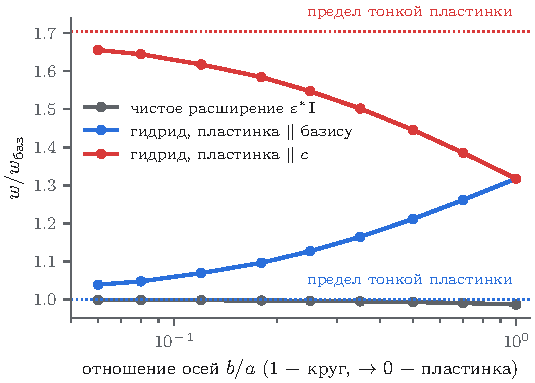
\includegraphics[width=0.66\linewidth]{f5_shape}
\caption{Упругая энергия эллиптического включения на единицу объёма от отношения осей, в единицах энергии тонкой
базисной пластинки. Точки --- расчёт методом Фурье (сетка $1024^2$). Серые --- чистое расширение: энергия от формы не
зависит, как и предсказывает Эшелби. Синие и красные --- несоответствие гидрида для пластинки, параллельной
базису и оси $c$; пунктир --- пределы тонкой пластинки.}
\label{fig:f5_shape}
\end{figure}

\section{Поле вокруг пластинки}

Внутри пластинки напряжения огромны --- гигапаскали (порядка $E\eps^*$). Но для соседей важнее поле \emph{снаружи}
(рис.~\ref{fig:f5_field}). Пластинка расширяется поперёк себя и раздвигает металл, как клин. Перед её торцами
матрица растянута: гидростатическое напряжение здесь доходит до сотен МПа. Над и под широкими гранями матрица
сжата.

\fig[0.75]{f5_field}{Гидростатическое напряжение в матрице вокруг тонкой пластинки $\delta$-гидрида (отношение
осей 0.1, нормаль вдоль $c$; расчёт методом Фурье, $E = 90$~ГПа). Красное --- растяжение, синее --- сжатие. У
торцов --- растяжение в сотни МПа.}

\begin{zrbox}
У торцов пластинки сходятся сразу два эффекта: туда стекается водород (глава~3), и там новой пластинке той же
ориентации выгоднее появиться --- её несоответствие «встраивается» в уже растянутую матрицу. Поэтому гидриды
растут цепочками торец к торцу, и из микропластинок складываются длинные макрогидриды. Над и под пластинкой
матрица сжата, и новые пластинки там зарождаются хуже. Насколько сильно одни пластинки влияют на зарождение
других --- один из ключевых и плохо известных параметров модели.
\end{zrbox}

\section{Работа внешнего напряжения}

Если тело нагружено однородным напряжением $\sigma^A$, появление включения меняет энергию системы дополнительно на
\begin{keyf}[Энергия взаимодействия с нагрузкой]
\[
\Delta G_{\text{вз}} = -\,\sigma^A_{ij}\,\eps^*_{ij}\,V .
\]
\end{keyf}
Этот результат тоже принадлежит Эшелби. Он точный и \emph{не зависит от формы} включения. Смысл простой:
нагрузка совершает работу на деформации превращения. Если включение расширяется вдоль растягивающей нагрузки,
работа положительна, и превращение облегчается.

Несоответствие гидрида связано с решёткой зерна, а не с формой пластинки. Поэтому нагрузка выбирает не форму, а
\emph{зёрна}: выгоднее всего выпадать в зёрнах, где ось $c$ (направление самого большого расширения, 7.2\,\%)
смотрит вдоль растяжения (рис.~\ref{fig:f5_orient}б). Пластинка в таком зерне лежит около базиса, то есть
\emph{поперёк} нагрузки. Именно так окружное напряжение в трубе рождает радиальные гидриды --- в тех зёрнах, чьи оси
$c$ близки к окружному направлению.

\begin{zrbox}
Сравним числа. Работа окружного напряжения 100~МПа: $\sigma\eps_c \approx 7$~МДж/м$^3$, то есть около 70~Дж на моль
водорода. Разница между лучшим и худшим зерном, $\sigma(\eps_c-\eps_a)$, --- всего 27~Дж/моль. Упругая
энергия самой пластинки --- около 3000~Дж/моль, движущая сила выпадения --- около 5000~Дж/моль. Нагрузка ---
поправка в один-два процента. Как такая малая поправка решает ориентацию, объясняет теория зарождения: работа
нагрузки входит в показатель экспоненты (глава~6).
\end{zrbox}

\section{Метод Фурье: как считает модель}
\label{sec:fourier}

Для многих пластинок произвольной формы аналитического решения нет. Его даёт метод, развитый Хачатуряном. Пусть
собственная деформация задана на периодической сетке: $\eps^*(\mathbf x) = \eps^{*0}\chi(\mathbf x)$, где $\chi$
равна 1 в гидриде и 0 в матрице. Уравнение равновесия $\partial_j\sigma_{ij} = 0$ с законом Гука после
преобразования Фурье становится \emph{алгебраическим}: для каждой гармоники $\mathbf k$
\begin{equation}
\hat{\mathbf u}(\mathbf k) = -i\,\mathbf N(\mathbf k)\,\bigl(\mathbf k\cdot\hat{\boldsymbol\tau}(\mathbf k)\bigr),
\qquad \hat{\boldsymbol\tau} = \mathbf C:\hat{\eps}^*,
\end{equation}
где $\mathbf N(\mathbf k) = (\mathbf k\cdot\mathbf C\cdot\mathbf k)^{-1}$ --- обратный «акустический» тензор. Для
изотропной среды
$N_{ij} = \dfrac{1}{\mu k^2}\Bigl(\delta_{ij} - \dfrac{\lambda+\mu}{\lambda+2\mu}\,n_in_j\Bigr)$, $\mathbf n = \mathbf k/k$.
Решение --- одно прямое и одно обратное быстрое преобразование Фурье, за $O(N\log N)$ операций для $N$ точек сетки.

У этого подхода есть красивое следствие. Упругая энергия выражается через форму включения и функцию направления
$B(\mathbf n)$:
\[
W = \frac{1}{2}\int B(\mathbf n)\,|\hat\chi(\mathbf k)|^2\,\frac{\dd^3k}{(2\pi)^3},\qquad
B(\mathbf n) = \boldsymbol\sigma^0:\eps^{*0} - \mathbf n\cdot\boldsymbol\sigma^0\cdot\mathbf N(\mathbf n)\cdot\boldsymbol\sigma^0\cdot\mathbf n,
\]
где $\boldsymbol\sigma^0 = \mathbf C:\eps^{*0}$. У тонкой пластинки спектр $\hat\chi$ сосредоточен вдоль её нормали,
и энергия на объём равна $B(\mathbf n)$ при нормали пластинки. Значит, \textbf{плоскость залегания --- та, чья нормаль
минимизирует $B(\mathbf n)$}. Это правило Хачатуряна; формула тонкой пластинки выше --- его частный случай.

\begin{exercise}
Повторите вывод энергии шара: внутри шара с чистым расширением полная деформация
$\eps^{\text{вн}} = \frac{1+\nu}{3(1-\nu)}\eps\,\mathbf I$. Найдите напряжение внутри и подставьте его в
$W = -\tfrac12 V\sigma^{\text{вн}}:\eps^*$.
\end{exercise}

\begin{exercise}
Выведите формулу энергии тонкой пластинки, считая, что в её плоскости полная деформация равна нулю, а поперёк
напряжения нет (плоское напряжённое состояние в пластинке).
\end{exercise}

\begin{exercise}
Посчитайте энергию тонкой пластинки для нормали под 15\textdegree{} к оси $c$. Сколько это на моль водорода, если
объём гидрида на моль водорода $10^{-5}$~м$^3$?
\end{exercise}

\begin{exercise}
Окружное напряжение 120~МПа, осевое 60~МПа (труба с заглушками). Найдите работу $\sigma^A:\eps^*$ на моль водорода для
зерна, у которого ось $c$ лежит вдоль окружного направления, и для зерна с осью $c$ по радиусу.
\end{exercise}

\chapter{Зарождение, рост и кинетика превращения}

\section{Гомогенное зарождение}

Пересыщенный раствор метастабилен (глава~2): гидрид выгоднее, но его ещё нужно создать. Пусть в растворе
флуктуацией возник шарик новой фазы радиуса $r$. Объём даёт выигрыш $\Delta g$ на единицу объёма (химическая
движущая сила минус упругая энергия несоответствия), а поверхность стоит $\gamma$ на единицу площади:
\begin{equation}
\Delta G(r) = -\tfrac43\pi r^3\,\Delta g + 4\pi r^2\,\gamma .
\end{equation}
При малых $r$ побеждает поверхность ($r^2$), при больших --- объём ($r^3$). Функция имеет максимум
(рис.~\ref{fig:f6_cnt}):
\begin{keyf}[Критический зародыш]
\[
r^* = \frac{2\gamma}{\Delta g},\qquad \Delta G^* = \frac{16\pi}{3}\,\frac{\gamma^3}{\Delta g^2}.
\]
\end{keyf}
Зародыши меньше $r^*$ растворяются чаще, чем растут; больше $r^*$ --- растут. Барьер $\Delta G^*$ обратно
пропорционален \emph{квадрату} движущей силы. Вдвое большее пересыщение снижает барьер вчетверо.

\begin{figure}[htbp]\centering
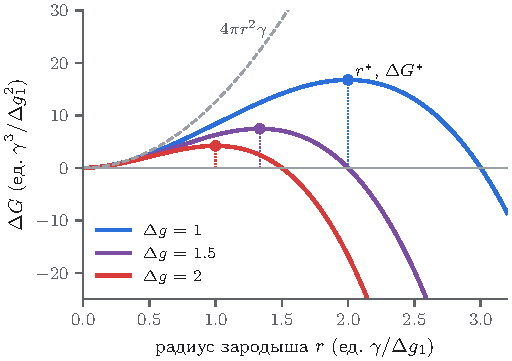
\includegraphics[width=0.6\linewidth]{f6_cnt}
\caption{Энергия зародыша от радиуса при трёх движущих силах. Точки --- критический радиус и барьер; с ростом
$\Delta g$ они быстро уменьшаются. Пунктир --- вклад поверхности.}
\label{fig:f6_cnt}
\end{figure}

\begin{zrbox}
Упругая энергия несоответствия $w$ вычитается из химической движущей силы: $\Delta g = \Delta g_{\text{хим}} - w$.
Если $w$ съедает большую часть $\Delta g_{\text{хим}}$, барьер огромен, и выпадения нет, пока раствор не пересытится
настолько, что $\Delta g_{\text{хим}}$ заметно превысит $w$. Это вторая сторона гистерезиса TSSD--TSSP из главы~2:
линия выпадения лежит там, где оставшаяся движущая сила $\Delta g_{\text{хим}} - w$ уже даёт заметную скорость
зарождения.
\end{zrbox}

\section{Скорость зарождения и С-кривые}

Число зародышей, появляющихся в единице объёма за единицу времени,
\begin{equation}
\dot N = N_s\,Z\,\beta^*\,\exp\Bigl(-\frac{\Delta G^*}{k_BT}\Bigr),
\end{equation}
где $N_s$ --- число мест для зарождения, $\beta^*$ --- частота присоединения атомов к критическому зародышу
(она пропорциональна $D$, то есть $e^{-Q/RT}$), $Z\sim0.01$--$0.1$ --- множитель Зельдовича (доля зародышей на
вершине барьера, которые всё-таки вырастут).

Два множителя тянут в разные стороны (рис.~\ref{fig:f6_rate}а). С переохлаждением движущая сила растёт, барьер
падает, и $e^{-\Delta G^*/kT}$ взлетает --- от нуля у $T_e$. Но с понижением температуры падает подвижность
$e^{-Q/RT}$. Их произведение имеет максимум. Если к скорости зарождения добавить скорость роста, получится время,
за которое превратится заданная доля, --- кривая в форме буквы С с «носом» на диаграмме
температура--время--превращение (рис.~\ref{fig:f6_rate}б).

\fig{f6_rate}{а) Скорость зарождения (чёрная) как произведение множителя барьера (красный, растёт с
переохлаждением) и подвижности (синий, падает при охлаждении). б) С-кривые начала (1\,\%) и конца (99\,\%)
превращения из тех же скоростей зарождения и роста (схема). Быстрее всего превращение идёт у «носа».}

\begin{idea}
Почему зарождение такое «пороговое»? Барьер стоит в показателе экспоненты и обычно в десятки $k_BT$. Если
$\Delta G^*/k_BT = 50$, то уменьшение барьера всего на 10\,\% (5$k_BT$) ускоряет зарождение в $e^5\approx150$ раз.
Поэтому при охлаждении зарождение почти не идёт, а затем в узком интервале температур начинается лавинообразно ---
это и видно как линия TSSP.
\end{idea}

\section{Неоднородное зарождение}

В реальном металле зародыш почти всегда появляется не в идеальном объёме, а на дефекте, который отдаёт часть своей
энергии. На границе зерна зародыш-линза заменяет кусок границы площадью $\pi a^2$ с энергией $\gamma_{\alpha\alpha}$
(рис.~\ref{fig:f6_het}а). Равновесие натяжений в точке стыка: $\gamma_{\alpha\alpha} = 2\gamma_{\alpha\beta}\cos\theta$.
Барьер уменьшается в $S(\theta)$ раз:
\begin{equation}
\frac{\Delta G^*_{\text{гр}}}{\Delta G^*_{\text{гом}}} = S(\theta) = \tfrac12(2+\cos\theta)(1-\cos\theta)^2 .
\end{equation}
Чем выше энергия границы по отношению к межфазной, тем меньше барьер (рис.~\ref{fig:f6_het}б). Ещё выгоднее
стыки трёх зёрен и их вершины. Мест на границах меньше, чем в объёме, но при малых переохлаждениях выигрыш в
барьере важнее числа мест.

\fig{f6_het}{а) Зародыш-линза на границе зерна; натяжения уравновешены при $\gamma_{\alpha\alpha} =
2\gamma_{\alpha\beta}\cos\theta$. б) Множитель барьера $S$ от отношения энергий границы и межфазной поверхности.}

Другие места неоднородного зарождения:
\begin{itemize}
\item \textbf{дислокации}: в растянутой области под краевой дислокацией несоответствие гидрида частично
  «скомпенсировано», и туда стекается водород (главы~3, 4);
\item \textbf{следы старых гидридов}: дислокационные петли и остаточная пластическая деформация после растворения
  (эффект памяти, глава~7);
\item \textbf{торцы уже растущих пластинок} --- там матрица растянута (глава~5).
\end{itemize}

\section{Форма зародыша}

Барьер для шара --- лишь приближение. Если межфазная энергия анизотропна (когерентная грань дешёвая, торцы
дорогие), а упругая энергия минимальна для тонкой пластинки (глава~5), выгоднее зародыш-диск. Для диска радиуса $a$
и толщины $2c$ с дешёвыми широкими гранями $\gamma_1$ и дорогими торцами $\gamma_2$ выигрыш тем больше, чем
сильнее $\gamma_2/\gamma_1$ и чем выгоднее тонкая форма упруго. Поэтому уже на стадии зарождения гидрид ---
тонкий когерентный диск на плоскости с наименьшей упругой энергией.

\section{Зарождение под напряжением}

Нагрузка добавляет к движущей силе работу $\sigma^A:\eps^*$ на единицу объёма гидрида (глава~5). Насколько это
сдвигает температуру выпадения? На линии выпадения при концентрации $C$ раствор пересыщен на
$RT\ln(C/C_e(T))$, а $C_e = Ae^{-Q/RT}$. Если работа нагрузки на моль водорода $W_\sigma = \sigma\eps^*V$
добавляется к движущей силе, то для той же скорости зарождения достаточно меньшего пересыщения, и выпадение
начнётся раньше на
\begin{keyf}[Сдвиг температуры выпадения]
\[
\delta T \approx \frac{T\,W_\sigma}{Q} = \frac{T\,\sigma\,\eps^*\,V}{Q}.
\]
\end{keyf}
Для гидрида ($T\approx580$~К, $\eps^* = 0.072$, $V = 10^{-5}$~м$^3$/моль H, $Q\approx32$~кДж/моль по наклону TSSP)
получается $\delta T/\sigma\approx0.013$~К/МПа. По измерениям на Zr--2.5Nb (Vizca\'{\i}no и др., 2014) сдвиг около
0.08~К/МПа --- в шесть раз больше. Значит, внешнее напряжение действует на зародыш сильнее, чем работа на его
среднем несоответствии. Возможные причины: концентрация напряжений у дефектов, где идёт зарождение;
пластичность; многоступенчатая природа зарождения. Это открытый вопрос, и в модели он отражён отдельным
параметром связи напряжений с зарождением.

\begin{figure}[htbp]\centering
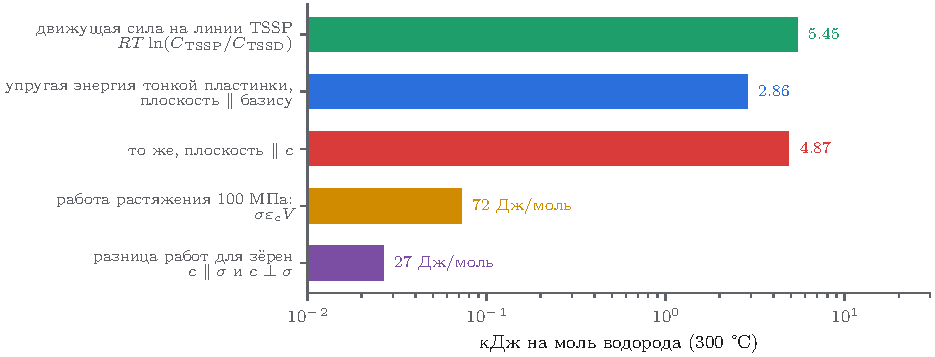
\includegraphics[width=0.85\linewidth]{f6_budget}
\caption{Энергетический бюджет выпадения гидрида на моль водорода при 300\degC{} для Э635 (логарифмическая шкала):
движущая сила на линии выпадения, упругая энергия тонкой пластинки на базисе и вдоль оси $c$, работа окружного
напряжения 100~МПа и разница этой работы между самым выгодным и самым невыгодным зерном.}
\label{fig:f6_budget}
\end{figure}

\begin{zrbox}
Почему крошечная работа решает ориентацию (рис.~\ref{fig:f6_budget})? После вычета упругой энергии у зародыша
остаётся $\Delta g\approx5.5-2.9\approx2.6$~кДж/моль~H. Работа 100~МПа --- 72~Дж/моль, то есть 2.8\,\% от этого
остатка. Барьер $\propto1/\Delta g^2$ уменьшается на $\approx5.5\,\%$. При барьере $50\,k_BT$ это $2.8\,k_BT$,
и скорость зарождения растёт примерно в 15 раз. Даже разница между зёрнами (27~Дж/моль) меняет скорость
примерно в 2.8 раза. В конкуренции зародышей такие множители решают, какие пластинки появятся первыми и заберут
водород.
\end{zrbox}

\section{Рост}

Зародыш, перешедший барьер, растёт. Гидрид богаче водородом, чем раствор, поэтому вокруг растущей пластинки
образуется обеднённая зона (рис.~\ref{fig:f6_growth}а). На границе --- равновесная концентрация $c_e$, вдали ---
исходная $c_0$. Если рост ограничен подводом водорода, граница движется со скоростью
\[
v = \frac{D}{c_\beta-c_e}\left.\frac{\partial c}{\partial x}\right|_{\text{гр}}\sim\frac{D}{c_\beta-c_e}\,\frac{c_0-c_e}{\sqrt{Dt}} .
\]
\begin{itemize}
\item \textbf{утолщение} широкой грани идёт по закону $\propto\sqrt{Dt}$: обеднённая зона перед ней расширяется, и
  подвод слабеет;
\item \textbf{удлинение} торца идёт с постоянной скоростью $\propto D(c_0-c_e)/r_{\text{торца}}$: острый торец всё
  время встречает свежий пересыщенный раствор (рис.~\ref{fig:f6_growth}б).
\end{itemize}

\fig{f6_growth}{а) Профиль концентрации у растущей пластинки: внутри --- состав гидрида $c_\beta$, на границе ---
равновесие $c_e$, вдали --- пересыщение $c_0$; обеднённая зона шириной $\sim\sqrt{Dt}$. б) Толщина растёт как
$\sqrt t$, длина --- линейно.}

Поэтому пластинки становятся всё более тонкими и длинными. Если рост ограничен не диффузией, а перестройкой
решётки на границе (\emph{рост, контролируемый границей}), скорость $v = M\,\Delta g$ определяется подвижностью
границы $M$ и не зависит от времени.

\section{Кинетика превращения в целом}

Если зародыши появляются со скоростью $\dot N$, а растут со скоростью $v$, то доля превращённого объёма $f(t)$
описывается уравнением Колмогорова--Джонсона--Мела--Аврами:
\begin{keyf}[Уравнение Аврами]
\[
f(t) = 1 - \exp\bigl(-(kt)^n\bigr).
\]
\end{keyf}
Вывод изящен. Сначала посчитаем «расширенный» объём, как если бы зёрна росли сквозь друг друга, не замечая
соседей: $f_{\text{расш}} = \int_0^t\dot N\,\tfrac43\pi v^3(t-\tau)^3\dd\tau\propto t^4$. Реальный прирост --- только
та часть, что попадает в ещё не превращённый объём: $\dd f = (1-f)\,\dd f_{\text{расш}}$. Отсюда
$f = 1-e^{-f_{\text{расш}}}$. Показатель $n$ говорит о механизме: 4 --- постоянное зарождение и трёхмерный рост,
3 --- все зародыши сразу, меньше --- рост в одном или двух измерениях или под контролем диффузии
(рис.~\ref{fig:f6_jmak}).

\fig{f6_jmak}{а) Кинетика Аврами при разных показателях $n$. б) В координатах $\ln(-\ln(1-f))$ против $\ln t$ ---
прямые с наклоном $n$; так показатель находят из опыта.}

\section{Огрубление и эффект Гиббса--Томсона}

У маленькой частицы велика доля поверхности, и её энергия на атом выше. Поэтому раствор вокруг неё равновесен
при большей концентрации:
\begin{equation}
c_r = c_\infty\exp\Bigl(\frac{2\gamma V}{rRT}\Bigr).
\end{equation}
Для гидрида при 300\degC{} и $\gamma=0.2$~Дж/м$^2$ частица радиусом 10~нм равновесна с раствором на 9\,\% богаче, чем
большая, а радиусом 1~нм --- вдвое (рис.~\ref{fig:f6_gt}). Водород течёт от мелких частиц к крупным: мелкие
растворяются, крупные растут. Это \textbf{огрубление} (созревание по Оствальду). Средний размер растёт как
$\bar r^3 - \bar r_0^3\propto t$ (теория Лифшица--Слёзова--Вагнера).

\begin{figure}[htbp]\centering
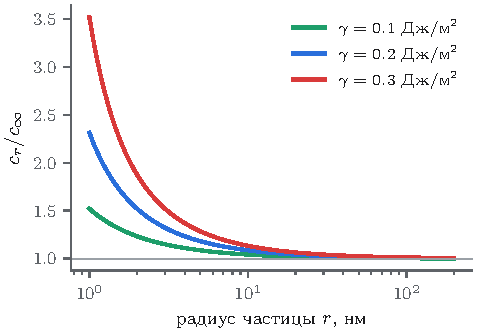
\includegraphics[width=0.58\linewidth]{f6_gt}
\caption{Эффект Гиббса--Томсона для гидрида при 300\degC: во сколько раз растворимость у частицы радиуса $r$ выше,
чем у плоской границы, при трёх энергиях межфазной границы.}
\label{fig:f6_gt}
\end{figure}

\begin{zrbox}
Для гидридов огрубление важно при выдержках у высоких температур: мелкие пластинки растворяются в пользу крупных.
Те же соображения объясняют, почему при нагреве первыми растворяются мелкие гидриды. А те, что остались
нерастворёнными на максимуме температуры, --- самые крупные. Они переживают цикл и задают, где выпадут новые
пластинки при охлаждении.
\end{zrbox}

\begin{exercise}
Выведите $r^*$ и $\Delta G^*$, приравняв нулю производную $\Delta G(r)$. Как изменится $\Delta G^*$, если движущая
сила уменьшится на 20\,\%?
\end{exercise}

\begin{exercise}
Покажите, что для линзы на границе зерна объём и площадь выражаются через объём шара того же радиуса кривизны и
множитель $S(\theta)$, и получите формулу $S(\theta)$.
\end{exercise}

\begin{exercise}
По формуле сдвига температуры выпадения оцените $\delta T$ для нагрузки 150~МПа. Сравните с шириной полосы гистерезиса
TSSD--TSSP.
\end{exercise}

\begin{exercise}
Выведите уравнение Аврами для случая, когда все зародыши появились в момент $t=0$ с плотностью $N$ и растут
трёхмерно со скоростью $v$. Какой получится показатель $n$?
\end{exercise}

\chapter{Пластичность, остаточные напряжения и текстура}

\section{Диаграмма растяжения}

Растянем образец (рис.~\ref{fig:f7_ss}). Сначала напряжение растёт пропорционально деформации с наклоном $E$ ---
это упругость: снимите нагрузку, и образец вернётся к исходной длине. Выше \textbf{предела текучести}
$\sigma_y$ начинается пластическое течение. Деформация после разгрузки уже не исчезает: разгрузка идёт по
прямой с тем же наклоном $E$, и остаётся пластическая деформация $\eps_p$. Чтобы деформировать металл дальше,
нужно всё большее напряжение --- это \textbf{упрочнение}.

\begin{figure}[htbp]\centering
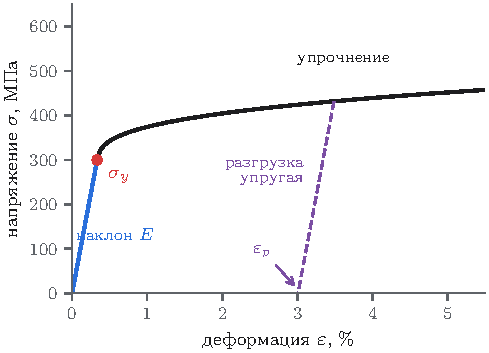
\includegraphics[width=0.6\linewidth]{f7_ss}
\caption{Схема диаграммы растяжения: упругий участок (наклон $E$), предел текучести $\sigma_y$, упрочнение;
разгрузка упругая, остаётся пластическая деформация $\eps_p$.}
\label{fig:f7_ss}
\end{figure}

Для оболочечных сплавов циркония при 300--400\degC{} предел текучести порядка 200--500~МПа: меньше у
рекристаллизованного металла, больше у холоднодеформированного и снятого от напряжений.

\section{Когда металл течёт при сложном нагружении}

В трубе напряжения не одноосные: под давлением окружное $\sigma_\theta$ вдвое больше осевого $\sigma_z$. Нужен
критерий текучести для любого напряжённого состояния. Гидростатическое давление на текучесть почти не влияет ---
дислокации двигает только касательное напряжение. Поэтому критерий строят по девиатору.
\begin{keyf}[Критерий Мизеса]
\[
\sigma_{\text{экв}} = \sqrt{\tfrac32\,s_{ij}s_{ij}}\;=\;\sigma_y
\]
(для плоского состояния $\sigma_1^2-\sigma_1\sigma_2+\sigma_2^2 = \sigma_y^2$).
\end{keyf}
Критерий Треска --- максимальное касательное напряжение $(\sigma_{\max}-\sigma_{\min})/2 = \sigma_y/2$. На плоскости
главных напряжений Мизес --- эллипс, Треска --- вписанный шестиугольник (рис.~\ref{fig:f7_yield}).

\begin{figure}[htbp]\centering
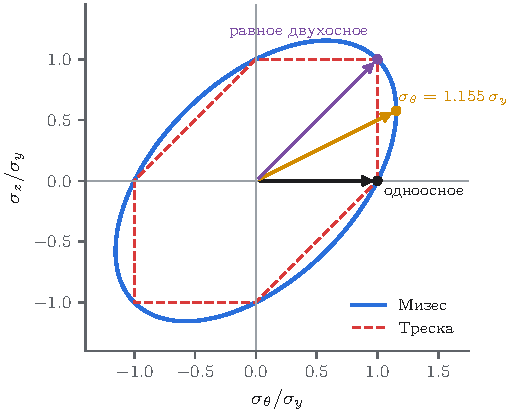
\includegraphics[width=0.52\linewidth]{f7_yield}
\caption{Поверхности текучести в плоскости $(\sigma_\theta,\sigma_z)$: Мизес (эллипс) и Треска (шестиугольник).
Стрелки --- пути нагружения: одноосное растяжение, труба с заглушками ($\sigma_z = \sigma_\theta/2$), равное
двухосное. Труба начинает течь при $\sigma_\theta\approx1.155\,\sigma_y$.}
\label{fig:f7_yield}
\end{figure}

\begin{idea}
Почему при $\sigma_z = \sigma_\theta/2$ труба выдерживает больше, чем стержень? Осевое растяжение уменьшает
девиатор: два растяжения частично «гасят» друг друга по сдвигу. Поэтому одинаковые окружные напряжения в
трубе и в кольце, растягиваемом в одном направлении, дают разную пластичность --- и разную переориентацию.
\end{idea}

\section{Дислокационная природа текучести}

Дислокация начинает скользить, когда касательное напряжение в её плоскости и направлении скольжения достигает
критического $\tau_c$. При одноосном растяжении это напряжение равно $\sigma\cos\varphi\cos\lambda$ (закон
Шмида; $\varphi$ и $\lambda$ --- углы нагрузки с нормалью к плоскости и с направлением скольжения). Упрочнение
возникает потому, что дислокации множатся и мешают друг другу: $\tau\approx\alpha\mu b\sqrt\rho$, где $\rho$ ---
плотность дислокаций (уравнение Тейлора).

В цирконии лёгкое скольжение одно --- призматическое $\{10\bar10\}\langle11\bar20\rangle$. Деформация вдоль оси $c$
требует пирамидального скольжения $\langle c+a\rangle$ (оно в несколько раз «твёрже») или двойникования. Поэтому
прочность зерна сильно зависит от того, как к нагрузке повёрнута ось $c$. Прочность трубы в целом зависит от
текстуры (раздел~\ref{sec:texture}). Анизотропную текучесть описывают критерием Хилла --- обобщением Мизеса с
разными весами для разных компонент напряжения.

\section{Пластическая аккомодация гидрида и память}

Упругие напряжения от гидрида --- порядка $\mu\eps^*\sim30~\text{ГПа}\cdot0.05\approx1.5$~ГПа. Это в несколько
раз выше предела текучести. Значит, вокруг всякого гидрида, кроме совсем мелкого, металл течёт. Оценим
размер пластической зоны для простейшей модели: жёсткий шар радиуса $a$ с линейным несоответствием $\delta$ в
идеально пластичной матрице (за зоной --- упругость, в зоне материал несжимаем). Объём, «выдавленный» шаром,
$4\pi a^3\delta$, должен равняться объёму, на который сдвигается упругая граница зоны радиуса $c$. Отсюда
\begin{keyf}[Пластическая зона вокруг включения]
\[
\Bigl(\frac{c}{a}\Bigr)^3 \approx \frac{6\mu\,\delta}{\sigma_y}.
\]
\end{keyf}
Для гидрида ($\mu = 33$~ГПа, $\delta\approx0.057$ --- треть объёмного несоответствия, $\sigma_y = 300$~МПа) зона в
3.4~раза больше самого гидрида (рис.~\ref{fig:f7_zone}). У настоящей пластинки зона вытянута вдоль неё и наиболее
сильна у торцов. Пластическое течение идёт рождением и выбросом дислокационных петель.

\fig{f7_zone}{а) Радиус пластической зоны вокруг несоразмерного включения в единицах его радиуса от предела
текучести матрицы при трёх несоответствиях. б) Схема: гидрид, пластический ореол и выброшенные дислокационные
петли.}

\begin{zrbox}
Пластическая аккомодация --- ключ к трём наблюдениям.
\begin{itemize}
\item \textbf{Гистерезис}: новый гидрид платит работой пластического течения, а при растворении эта работа не
  возвращается. Отсюда часть разрыва между TSSP и TSSD (глава~2).
\item \textbf{Память}: при растворении гидрида дислокации и остаточная деформация остаются. При следующем
  охлаждении гидрид выпадает там же --- места уже «подготовлены». Сколько памяти переживает выдержку при
  максимальной температуре, зависит от отжига (возврата) и проверяется опытами с многократными циклами.
\item \textbf{Коллективная пластичность}: когда гидридов много, их пластические зоны сливаются, и металл вокруг
  целой пачки пластинок течёт как одно целое. Это меняет поле напряжений, в котором зарождаются соседи.
\end{itemize}
\end{zrbox}

\section{Остаточные и межзёренные напряжения}

Даже без внешней нагрузки металл не свободен от напряжений. Их различают по масштабу:
\begin{itemize}
\item \textbf{I рода} --- на масштабе детали (после прокатки, сварки, изгиба);
\item \textbf{II рода} --- между зёрнами. В цирконии их создаёт анизотропия: при охлаждении зерно сжимается вдоль
  $c$ сильнее, чем поперёк, а соседи с другой ориентацией ему мешают. Оценка $\Delta\alpha\,\Delta T\,E$ даёт
  десятки МПа --- сопоставимо с нагрузками, при которых идёт переориентация;
\item \textbf{III рода} --- на масштабе дислокаций и включений (поле вокруг гидрида, глава~5).
\end{itemize}

\begin{zrbox}
Межзёренные напряжения разные в разных зёрнах, и каждое зерно «видит» внешнюю нагрузку со своей добавкой. Это
даёт разброс условий зарождения от зерна к зерну. Его величина --- один из параметров модели.
\end{zrbox}

\section{Текстура трубы}
\label{sec:texture}

Ориентации зёрен в трубе не случайны. Прокатка и отжиг выстраивают их так, что оси $c$ большинства зёрен лежат
в плоскости радиус--окружность и наклонены от радиального направления к окружному на $\pm(30$--$40)^\circ$. Это
\textbf{текстура}. Её изображают \textbf{полюсной фигурой}: стереографической проекцией, на которой отмечены
направления осей $c$ всех зёрен (рис.~\ref{fig:f7_texture}а).

Для гидридов удобна свёртка текстуры в три числа --- \textbf{факторы Кернса}:
\begin{keyf}[Факторы Кернса]
\[
f_d = \bigl\langle\cos^2\angle(\mathbf c,\mathbf d)\bigr\rangle_{\text{по объёму}},\qquad f_r+f_\theta+f_z = 1 .
\]
\end{keyf}
$f_r$ --- доля «ориентированности» осей $c$ по радиусу, $f_\theta$ --- по окружности, $f_z$ --- вдоль оси трубы. Для
типичных оболочек $f_r\approx0.5$--$0.7$, $f_\theta\approx0.25$--$0.35$, $f_z\approx0.05$--$0.1$.

\fig{f7_texture}{Схема текстуры трубы: оси $c$ наклонены от радиального направления к окружному на
$\pm35^\circ$ с разбросом $12^\circ$. а) Полюсная фигура (0002) в равноплощадной проекции, центр --- радиальное
направление. б) Факторы Кернса этого распределения.}

\begin{zrbox}
Теперь всё складывается. Гидрид ложится около базисной плоскости своего зерна (глава~5). В трубе с радиальной
текстурой базисные плоскости большинства зёрен лежат примерно вдоль окружности, поэтому без нагрузки гидриды
\emph{окружные}. Окружное напряжение облегчает выпадение в зёрнах, у которых ось $c$ ближе к окружному
направлению (глава~5): в них пластинка встаёт по радиусу. Таких зёрен немного --- им соответствует $f_\theta$.
Поэтому переориентация зависит от текстуры. Дополнительный путь дают межзёренные гидриды и цепочки
пластинок, переходящие из зерна в зерно.
\end{zrbox}

\section{Итог: из чего складывается переориентация}

Соберём главы вместе.
\begin{enumerate}
\item \textbf{Сколько выпадет и когда} --- линии растворимости TSSD и TSSP, гистерезис между ними (главы~1, 2).
\item \textbf{Где окажется водород} --- быстрая диффузия выравнивает концентрацию на масштабе зёрен. Водород
  стекается к растянутым местам: торцам пластинок, вершинам трещин (глава~3).
\item \textbf{Какой формы и в какой плоскости} --- тонкие пластинки около базиса: так меньше упругая энергия
  несоответствия (главы~4, 5).
\item \textbf{В каких зёрнах и когда зародится} --- барьер зарождения, в показатель которого входят упругая
  энергия, работа нагрузки, дефекты и границы (главы~5, 6).
\item \textbf{Как пластинки выстраиваются} --- поле соседей, пластическая аккомодация, память о прежних гидридах
  (главы~5, 7).
\item \textbf{Какая доля станет радиальной} --- конкуренция зёрен с разной ориентацией, то есть текстура (глава~7).
\end{enumerate}
Модель гидридов --- это численная реализация всех шести пунктов одновременно. Читать её код и учебник по ней
(\texttt{../textbook}) после этого фундамента должно быть заметно легче.

\begin{exercise}
Найдите окружное напряжение начала текучести трубы с заглушками по Мизесу и по Треска. Насколько они различаются?
\end{exercise}

\begin{exercise}
Выведите оценку размера пластической зоны $(c/a)^3 = 6\mu\delta/\sigma_y$. Для этого возьмите упругое решение
$u = B/r^2$ вне зоны, условие текучести на её границе и несжимаемость внутри.
\end{exercise}

\begin{exercise}
Оси $c$ всех зёрен лежат в плоскости радиус--окружность под углом $\pm\chi$ к радиусу. Найдите $f_r$ и $f_\theta$.
При каком $\chi$ они равны?
\end{exercise}

\appendix
\renewcommand{\thechapter}{\Asbuk{chapter}}
\chapter{Справочные величины для Zr--H}

Значения --- ориентиры для оценок; для расчётов конкретного сплава берите его собственные измерения.

\begin{center}\footnotesize
\renewcommand{\arraystretch}{1.25}
\begin{tabularx}{\linewidth}{>{\raggedright\arraybackslash}p{4.3cm}>{\raggedright\arraybackslash}p{5.6cm}>{\raggedright\arraybackslash}X}
\toprule
величина & значение & источник, комментарий \\
\midrule
решётка $\alpha$-Zr (ГПУ) & $a = 0.323$~нм, $c = 0.515$~нм, $c/a = 1.593$ & комнатная температура \\
превращение $\alpha\to\beta$ в чистом Zr & 863\degC & \\
$\delta$-гидрид & ГЦК, ZrH$_{1.5\ldots1.7}$, $a\approx0.478$~нм & \\
ориентационное соотношение & $(0001)_\alpha\parallel\{111\}_\delta$ & плоскость залегания около $\{10\bar17\}$ (Westlake, 1968) \\
несоответствие $\delta$-гидрида & $\eps_a\approx0.046$, $\eps_c\approx0.072$, объём $\approx17\,\%$ & Carpenter (1973) \\
водород в гидриде & $\approx18\,000$~ppm (ZrH$_{1.66}$) & \\
объём гидрида на моль H & $\approx1.0\cdot10^{-5}$~м$^3$ & из плотности ZrH$_{1.66}$ \\
TSSD, Э635 & $\lg C[\text{ppm}] = 5.56 - 2240/T$ & ДСК, Плясов и др. (2023); $Q\approx43$~кДж/моль \\
TSSP, Э635 & $\lg C[\text{ppm}] = 5.08 - 1680/T$ & то же; $Q\approx32$~кДж/моль; зависит от режима \\
эвтектоид $\beta\to\alpha+\delta$ & $\approx550$\degC, $\approx6$~ат.\,\% H в $\alpha$ & Zuzek и др. (1990) \\
диффузия H в $\alpha$-Zr & $D = 7.9\cdot10^{-7}e^{-44.4~\text{кДж}/RT}$~м$^2$/с & Kearns (1972) \\
парциальный мольный объём H & $\bar V_{\mathrm H}\approx1.7$~см$^3$/моль & \\
упругость Zr (300--400\degC) & $E\approx80$--90~ГПа, $\nu\approx0.34$, $\mu\approx30$--33~ГПа & изотропное приближение \\
предел текучести оболочки (300--400\degC) & 200--500~МПа & от состояния (рекр./СОН) \\
энергия межфазной границы гидрида & $\sim0.1$--0.3~Дж/м$^2$ & плохо известна; параметр моделей \\
сдвиг выпадения под нагрузкой & $\approx0.08$~К/МПа & Zr--2.5Nb (Vizca\'{\i}no и др., 2014) \\
факторы Кернса оболочек & $f_r\approx0.5$--0.7, $f_\theta\approx0.25$--0.35 & \\
\bottomrule
\end{tabularx}
\end{center}

\section*{Перевод единиц}
\begin{itemize}
\item ppm (масс.) $\to$ ат.\,\%: $x = \dfrac{C/1.008}{C/1.008 + 10^6/91.22}$; 100~ppm $\approx0.9$~ат.\,\%.
\item $RT$ при 300\degC: 4.76~кДж/моль; $k_BT = 0.049$~эВ. 1~эВ на атом = 96.5~кДж/моль.
\item 1~МПа = 1~МДж/м$^3$; на моль водорода в гидриде: 1~МДж/м$^3$ $\approx10$~Дж/моль~H.
\end{itemize}

\chapter{Ответы и подсказки к упражнениям}

\subsection*{Глава 1}
\textbf{1.1.} $\Delta G = \Delta H\Delta T/T_e$: 100 и 1000~Дж/моль. $RT$ при 990 и 900~К --- 8.2 и 7.5~кДж/моль, то есть
движущая сила меньше $RT$ в 82 и 7.5 раза.
\textbf{1.2.} $\exp\bigl[\frac{Q}{R}\bigl(\frac1{573}-\frac1{673}\bigr)\bigr] = \exp(3.74)\approx42$.
\textbf{1.3.} Вдоль линии равновесия $\dd G_\alpha = \dd G_\beta$, то есть $V_\alpha\dd p - S_\alpha\dd T = V_\beta\dd p -
S_\beta\dd T$, откуда $\dd p/\dd T = \Delta S/\Delta V = \Delta H/(T\Delta V)$. Для напряжения роль $-p\,\dd V$ играет работа
$V\sigma:\dd\eps$, и $\dd T/\dd\sigma = T\eps^*V/\Delta H$ --- формула главы~6.

\subsection*{Глава 2}
\textbf{2.1.} $\mu_B = G - (X-1)\,\partial G/\partial X$ даёт $G_B + \Omega(1-X)^2 + RT\ln X$.
\textbf{2.2.} $Q = 2.24\cdot10^3\cdot\ln10\cdot R \approx 42.9$~кДж/моль. $T = 2240/(5.56-\lg C)$: 100~ppm --- 356\degC,
300~ppm --- 453\degC, 600~ppm --- 532\degC (почти эвтектоид).
\textbf{2.3.} $\Delta g = R\ln10\,(560 - 0.48\,T)$~Дж/моль: 6.4~кДж/моль при 200\degC, 5.5 при 300\degC, 4.5 при
400\degC. Падает с температурой: при высокой $T$ пластичность и возврат легче, и матрица «берёт» с гидрида меньше.
\textbf{2.4.} $C_\TSSD(400\degC)\approx171$~ppm растворено; около 129~ppm остаётся в гидридах. Выпадение начнётся на TSSP
при 171~ppm: $T = 1680/(5.08-\lg171)\approx 317\degC$.

\subsection*{Глава 3}
\textbf{3.1.} $D(350\degC)\approx1.5\cdot10^{-10}$~м$^2$/с. $t\sim L^2/D$: для 0.65~мм около 50~мин, для 50~мкм около 17~с.
\textbf{3.2.} $\mathbf J = 0$ при $\nabla\ln c = (\bar V/RT)\nabla\sigma_h$. При 600~МПа и 300\degC: $e^{0.21}\approx1.24$.
\textbf{3.3.} $g = 1 - 4r\sin^2(k\Delta x/2)$; $|g|\le1$ при $r\le1/2$.

\subsection*{Глава 4}
\textbf{4.1.} $\operatorname{tg}\varphi = 1.1547\cdot1.593/7 = 0.263$, $\varphi\approx14.7^\circ$.
\textbf{4.2.} $1.17^{1/3}-1\approx0.054$; дислокация примерно через каждые 18 плоскостей.
\textbf{4.3.} $\mu b^2/2\approx1.7\cdot10^{-9}$~Дж/м, то есть около 3.5~эВ на межатомное расстояние.

\subsection*{Глава 5}
\textbf{5.1.} $\sigma^{\text{вн}} = 3K(s-1)\eps\,\mathbf I$, $s = \frac{1+\nu}{3(1-\nu)}$; $W = \frac92K(1-s)\eps^2V = \frac{E}{1-\nu}\eps^2V$.
\textbf{5.2.} В пластинке $\eps^{\text{полн}}_{tt} = \eps^{\text{полн}}_{ss} = 0$, $\sigma_{nn} = \sigma_{nt} = \sigma_{ns} = 0$:
плоское напряжённое состояние с упругой деформацией $-\eps^*$ в плоскости; $w = \frac12\sigma:\eps_{\text{упр}}$.
\textbf{5.3.} $\eps_{tt} = 0.0476$; $w\approx297$~МДж/м$^3$, около 3.0~кДж/моль~H.
\textbf{5.4.} Ось $c$ по окружности: $(120\cdot0.072 + 60\cdot0.046)\cdot10 \approx 114$~Дж/моль. Ось $c$ по радиусу:
$(120\cdot0.046 + 60\cdot0.046)\cdot10\approx 82$~Дж/моль.

\subsection*{Глава 6}
\textbf{6.1.} $r^* = 2\gamma/\Delta g$, $\Delta G^* = 16\pi\gamma^3/(3\Delta g^2)$; при $\Delta g\to0.8\Delta g$ барьер растёт в
$1/0.64\approx1.56$ раза.
\textbf{6.2.} Объём линзы $V = \frac43\pi R^3 S(\theta)$, площадь межфазной поверхности и заменённой границы дают тот же
множитель в барьере.
\textbf{6.3.} $\delta T\approx0.013\cdot150\approx2$~К по упругой оценке, $\approx12$~К по измеренному сдвигу; полоса гистерезиса ---
около 80~К.
\textbf{6.4.} $f_{\text{расш}} = N\frac43\pi v^3t^3$, $n = 3$.

\subsection*{Глава 7}
\textbf{7.1.} Мизес: $\sigma_\theta = 2\sigma_y/\sqrt3\approx1.155\sigma_y$; Треска ($\sigma_r\approx0$): $\sigma_\theta = \sigma_y$; разница 15\,\%.
\textbf{7.2.} $\sigma_{rr} = -4\mu B/r^3$, $\sigma_{\theta\theta} = 2\mu B/r^3$; текучесть на $r = c$: $6\mu B/c^3 = \sigma_y$;
несжимаемость: $a^2u(a) = c^2u(c) = B$, $u(a) = \delta a$.
\textbf{7.3.} $f_r = \cos^2\chi$, $f_\theta = \sin^2\chi$; равны при $\chi = 45^\circ$.

\chapter{Что читать дальше}
\sloppy

Здесь собраны источники, на которых держится этот текст, и книги для углубления. Выходные данные проверяйте по
DOI или каталогу перед цитированием.

\subsection*{Материаловедение и физика твёрдого тела в целом}
\begin{itemize}
\item Askeland D.R., Fulay P.P., Wright W.J. \emph{The Science and Engineering of Materials}. 6th ed., Cengage, 2010 ---
  обзорный учебник; по нему сверялся охват частей I, II и IV этого текста (строение, диаграммы, механические свойства).
\item Callister W.D., Rethwisch D.G. \emph{Materials Science and Engineering: An Introduction}. Wiley (любое из поздних изданий).
\item Гуляев А.П. «Металловедение». М.: Металлургия; Новиков И.И. «Теория термической обработки металлов».
\item Kittel C. \emph{Introduction to Solid State Physics}. 8th ed., Wiley, 2005 (есть русские переводы ранних изданий);
  Ashcroft N.W., Mermin N.D. \emph{Solid State Physics}. 1976 (рус. пер.: «Физика твёрдого тела», Мир, 1979).
\end{itemize}

\subsection*{Кристаллография, дифракция, микроскопия}
\begin{itemize}
\item Cullity B.D., Stock S.R. \emph{Elements of X-Ray Diffraction}. 3rd ed., Prentice Hall, 2001.
\item Горелик С.С., Скаков Ю.А., Расторгуев Л.Н. «Рентгенографический и электронно-оптический анализ». М.: МИСиС.
\item Kelly A., Knowles K.M. \emph{Crystallography and Crystal Defects}. 2nd ed., Wiley, 2012.
\item Goldstein J.I. и др. \emph{Scanning Electron Microscopy and X-Ray Microanalysis}. 4th ed., Springer, 2018;
  Williams D.B., Carter C.B. \emph{Transmission Electron Microscopy}. 2nd ed., Springer, 2009.
\item Schwartz A.J. и др. (ред.) \emph{Electron Backscatter Diffraction in Materials Science}. 2nd ed., Springer, 2009.
\end{itemize}

\subsection*{Механика и разрушение}
\begin{itemize}
\item Dieter G.E. \emph{Mechanical Metallurgy}. McGraw-Hill, 1986; Золоторевский В.С. «Механические свойства металлов».
\item Anderson T.L. \emph{Fracture Mechanics: Fundamentals and Applications}. 4th ed., CRC Press, 2017.
\item Humphreys F.J., Hatherly M. \emph{Recrystallization and Related Annealing Phenomena}. 2nd ed., Elsevier, 2004.
\item Tenckhoff E. \emph{Deformation Mechanisms, Texture, and Anisotropy in Zirconium and Zircaloy}. ASTM STP 966, 1988 ---
  скольжение, двойникование и текстура именно в цирконии.
\end{itemize}

\subsection*{Фундамент}
\begin{itemize}
\item Porter D.A., Easterling K.E., Sherif M.Y. \emph{Phase Transformations in Metals and Alloys}. 3rd ed., CRC Press, 2009 ---
  главы 1--5 покрывают главы~\ref{ch:gibbs}--\ref{ch:diagrams}, \ref{ch:diffusion}, \ref{ch:defects} и \ref{ch:nucleation} этого текста подробнее.
\item Christian J.W. \emph{The Theory of Transformations in Metals and Alloys}. Pergamon, 2002 (русский перевод: «Теория
  превращений в металлах и сплавах», Мир).
\item Hillert M. \emph{Phase Equilibria, Phase Diagrams and Phase Transformations}. Cambridge, 2008.
\item Shewmon P. \emph{Diffusion in Solids}; Mehrer H. \emph{Diffusion in Solids}. Springer, 2007.
\item Hull D., Bacon D.J. \emph{Introduction to Dislocations}. 5th ed., 2011; Kelly A., Knowles K.M.
  \emph{Crystallography and Crystal Defects}. 2012.
\item Штремель М.А. «Прочность сплавов», ч.~I--II.
\end{itemize}

\subsection*{Упругость включений и микромеханика}
\begin{itemize}
\item Eshelby J.D. The determination of the elastic field of an ellipsoidal inclusion, and related problems.
  \emph{Proc. R. Soc. A} 241 (1957) 376.
\item Mura T. \emph{Micromechanics of Defects in Solids}. 1987.
\item Хачатурян А.Г. «Теория фазовых превращений и структура твёрдых растворов». Наука, 1974
  (англ.: \emph{Theory of Structural Transformations in Solids}, 1983).
\item Moulinec H., Suquet P. \emph{Comput. Methods Appl. Mech. Eng.} 157 (1998) 69 --- решатель на FFT.
\end{itemize}

\subsection*{Пластичность и текстура}
\begin{itemize}
\item Hill R. \emph{The Mathematical Theory of Plasticity}. Oxford, 1950.
\item Kocks U.F., Tom\'e C.N., Wenk H.-R. \emph{Texture and Anisotropy}. Cambridge, 1998.
\item Engler O., Randle V. \emph{Introduction to Texture Analysis}. 2nd ed., CRC Press, 2010; Bunge H.-J.
  \emph{Texture Analysis in Materials Science}. Butterworths, 1982.
\item Bachmann F., Hielscher R., Schaeben H. Texture analysis with MTEX. \emph{Solid State Phenomena} 160 (2010) 63.
\item Kearns J.J. WAPD-TM-472 (1965); \emph{J. Nucl. Mater.} 299 (2001) 171 --- факторы Кернса.
\end{itemize}

\subsection*{Водород и гидриды циркония}
\begin{itemize}
\item Puls M.P. \emph{The Effect of Hydrogen and Hydrides on the Integrity of Zirconium Alloy Components}. Springer, 2012.
\item Motta A.T. и др. Hydrogen in zirconium alloys: A review. \emph{J. Nucl. Mater.} 518 (2019) 440.
\item Bair J., Asle Zaeem M., Tonks M. A review on hydride precipitation in zirconium alloys. \emph{J. Nucl. Mater.} 466 (2015) 12.
\item Zuzek E., Abriata J.P., San-Martin A., Manchester F.D. The H--Zr system. \emph{Bull. Alloy Phase Diagrams} 11 (1990) 385.
\item Kearns J.J. \emph{J. Nucl. Mater.} 22 (1967) 292 --- растворимость; 43 (1972) 330 --- диффузия.
\item Carpenter G.J.C. \emph{J. Nucl. Mater.} 48 (1973) 264 --- несоответствие гидрида; Westlake D.G. \emph{J. Nucl. Mater.} 26 (1968) 208 --- плоскости залегания.
\item Puls M.P. \emph{Acta Metall.} 29 (1981) 1961 --- гистерезис растворимости.
\item Займовский А.С., Никулина А.В., Решетников Н.Г. «Циркониевые сплавы в ядерной энергетике». 1994.
\item Qin W. и др. \emph{Acta Mater.} 59 (2011) 7010; Wang S., Giuliani F., Britton T.B. \emph{Acta Mater.} 169 (2019) 76 ---
  межзёренные гидриды.
\item Vizca\'{\i}no P. и др. \emph{J. Nucl. Mater.} 447 (2014) 82 --- выпадение под нагрузкой.
\item Плясов А.А. и др. \emph{Physics of Atomic Nuclei} 86(12) (2023); Ядерная физика и инжиниринг 14(1) (2023) 12 ---
  переориентация и растворимость в Э635.
\end{itemize}

\end{document}
